\documentclass[hidelinks,12pt,a4paper,twoside]{article}

%% ==================================================================
%%%% Preamble
%% ==================================================================
%% ==================================================================
%%%% Packages
%% ==================================================================
\usepackage[a4paper]{geometry}
\usepackage[utf8]{inputenc}
\usepackage[ngerman]{babel}
\usepackage[T1]{fontenc}
\usepackage{newpxtext,newpxmath}
\usepackage[hidelinks]{hyperref}
\usepackage{amsmath,amssymb,amstext}
\usepackage{mathtools}
\usepackage[style=authoryear-ibid,backend=biber]{biblatex}
\usepackage{csquotes}
\usepackage{fancyhdr}
\usepackage{microtype}
\usepackage{graphicx}
\usepackage{float}
\usepackage{minted}
\usepackage{acronym}
\usepackage{booktabs}
\usepackage{multirow}
\usepackage{pgf}
\usepackage{pgfplots}
\usepackage{siunitx}
\usepackage{xcolor,mdframed}
\usepackage{lipsum}


%% ==================================================================
%%%% General Document Settings
%% ==================================================================
\linespread{1.5}
\parindent 0ex

\bibliography{bibliography.bib}

\graphicspath{ {./images/} }

\setcounter{tocdepth}{5}
\setcounter{secnumdepth}{5}

\sisetup{locale = DE}

\setminted{mathescape,
  linenos,
  numbersep=5pt,
  gobble=2,
  frame=lines,
  framesep=2mm}


%% ==================================================================
%%%% Fancy Header Settings
%% ==================================================================
\pagestyle{fancy}
\fancyhead{}
\fancyfoot{}
\fancyhead[L]{\MakeUppercase{}}
\fancyfoot[C]{\thepage}
\fancyhead[R]{\MakeUppercase{\leftmark}}

\setlength{\headheight}{15pt}


%% ==================================================================
%%%% Important Info Block
%% ==================================================================
\newenvironment{important}[1][]{%
   \begin{mdframed}[%
      backgroundcolor={red!15}, hidealllines=true,
      skipabove=0.7\baselineskip, skipbelow=0.7\baselineskip,
      splitbottomskip=2pt, splittopskip=4pt, #1]%
   \makebox[0pt]{% ignore the withd of !
      \smash{% ignor the height of !
         \fontsize{32pt}{32pt}\selectfont% make the ! bigger
         \hspace*{-19pt}% move ! to the left
         \raisebox{-2pt}{% move ! up a little
            {\color{red!70!black}\sffamily\bfseries !}% type the bold red !
         }%
      }%
   }%
}{\end{mdframed}}



\begin{document}

%% ==================================================================
%%%% Main Content
%% ==================================================================

\begin{center}
  \vspace*{1cm}
  \line(1,0){400}\\[1mm]
  \huge{\textbf{DIPLOMARBEIT}}\\[2mm]
  \large{\textbf{Advanced Parking Monitoring (APM)}}\\[1mm]
  \line(1,0){400}\\[2cm]
  Philipp Kraft, Dennis Köb und Samuel Bleiner\\[2mm]
  Dipl.-Ing. Christoph Stüttler \\[5mm]
  \today, Rankweil
  \vfill
\end{center}



\fancyfoot[LO,RE]{\sectionauthors}

\frontmatter

\section*{Eidesstattliche Erklärung}
\addcontentsline{toc}{section}{Eidesstattliche Erklärung}
Ich erkläre an Eides statt, dass ich die vorliegende Diplomarbeit selbständig und ohne fremde Hilfe verfasst, andere als die angegebenen Quellen und Hilfsmittel nicht benutzt und die den benutzten Quellen wörtlich und inhaltlich entnommenen Stellen als solche erkenntlich gemacht habe.

\vspace*{2cm}


\begin{center}
\begin{tabular}{cp{2em}c} 
   \hspace{4cm}        & & \hspace{6cm} \\\cline{1-1}\cline{3-3}
                       & & \\[-3mm]
   {\footnotesize Ort, Datum }  & & {\footnotesize Philipp Kraft}
\end{tabular}

\vspace*{1cm}

\begin{tabular}{cp{2em}c} 
   \hspace{4cm}        & & \hspace{6cm} \\\cline{1-1}\cline{3-3}
                       & & \\[-3mm]
   {\footnotesize Ort, Datum }  & & {\footnotesize Dennis Köb}
\end{tabular}

\vspace*{1cm}

\begin{tabular}{cp{2em}c} 
   \hspace{4cm}        & & \hspace{6cm} \\\cline{1-1}\cline{3-3}
                       & & \\[-3mm]
   {\footnotesize Ort, Datum }  & & {\footnotesize Samuel Brugger}
\end{tabular}

\end{center}

\cleardoublepage

\pagebreak


\section*{Kurzfassung}
\addcontentsline{toc}{section}{Kurzfassung}
In der nachfolgenden Arbeit wird ein System vorgestellt, welches die Parkplatzverwaltung und -überwachung vereinfachen soll. 
Um zu erreichen, dass diese Lösung modular und individuell auf jedem Parkplatz eingesetzt werden kann, werden zwei eigenständige Module, 
eines für die Kennzeichenerkennung und eines für die Fahrzeugerkennung, entwickelt. Diese Module sollen ihre Daten auf eine Datenbank 
hochladen können, welche dann über eine intuitive Web-Applikation verwaltet werden kann. Mithilfe der Kennzeichenerkennung sollen die 
unterschiedlichen Fahrzeuge eindeutig identifiziert werden und damit auch der Status des Fahrzeuges auf dem Parkplatz überwacht werden können. 
Die Fahrzeugerkennung detektiert den Status einer einzelnen Parklücke und dadurch kann überwacht werden welche Parklücke besetzt ist und welche 
nicht. Diese Daten werden in der Web-Applikation anschaulich dargestellt, welche neben umfangreichen Darstellungsmöglichkeiten auch eine eigene 
Benutzeroberfläche für Parkplatzbetreiber und Nutzer bietet. Dieses System ist durch seinen modularen Aufbau in der Lage sowohl Firmenparkplätze 
als auch öffentliche Parkplätze jeglicher Größe zu bedienen.
\pagebreak


\section*{Abstract}
\addcontentsline{toc}{section}{Abstract}
In the following paper, a system is presented, which shall improve parking lot
surveillance and management. To make sure that this solution can be used
individually on every kind of parking lot, there will be developed two
independent modules, one for license plate detection and one for vehicle
detection. These modules shall be able to send their data to a database, which
can be accessed and controlled via an intuitive web application. With the
license plate detection, it shall be possible to identify each vehicle and watch
their status on the parking lot. The vehicle detection detects the status of
each parking spot and therefore it can be monitored which parking spot is
currently taken and which is free to be used. These data are visualized in the
web application, which offers extensive display options as well as different
user interfaces for parking lot owners and customers. Through its modular
structure, the system can provide great service for company parking lots and
public parking lots of any size.
\pagebreak


\section*{Vorwort}
\addcontentsline{toc}{section}{Vorwort}
In den Jahren unserer Ausbildungszeit ist uns immer wieder aufgefallen, dass viele öffentliche gebührenpflichtige Parkplätze nicht mit neuen Innovationen betrieben werden. 
Daraufhin haben wir uns durch zusätzliche Anregung von unserem Betreuungslehrer Dipl.-Ing. Christoph Stüttler dazu entschieden diese Thematik für unsere Diplomarbeit heranzuziehen.
\\ \\
Diese Diplomarbeit soll aufzeigen wie eine modernes System zur Parkplatzverwaltung aussehen könnte. Es werden in dieser Arbeit verschiedene Themenbereiche wie Webinterfaces, künstliche Intelligenz und Mikrokontroller behandelt.
\pagebreak


\section*{Danksagung}
\addcontentsline{toc}{section}{Danksagung}
Ein lesenswertes Buch ist \citetitle{einstein}\footcite{einstein}
\pagebreak


\mainmatter
\setcounter{page}{1}


\tableofcontents
\pagebreak


\section{Projektteam}
\begin{figure}[htbp]
  \centering
  \begin{minipage}[t]{0.35\linewidth}
      \centering
      \includegraphics[width=\linewidth]{Philipp.png}
      \caption*{\textbf{Philipp Kraft}\\ \href{mailto:mail@philipp-kraft.com}{E-Mail: Mail@Philipp-Kraft.com}}
  \end{minipage}
  \hfill
  \begin{minipage}[t]{0.35\linewidth}
      \centering
      \includegraphics[width=\linewidth]{Dennis.png}
      \caption*{\textbf{Dennis Köb}\\ \href{mailto:dennis.koeb@gmail.com}{E-Mail: Dennis.Koeb@gmail.com}}
  \end{minipage}
\end{figure}

\begin{figure}[H]
  \centering
  \frame{\includegraphics[width=0.35\linewidth]{Samuel.png}}
  \caption*{\textbf{Samuel Bleiner}\\ \href{mailto:bleiner.samuel@gmail.com}{E-Mail: Bleiner.Samuel@gmail.com}}
\end{figure}
\pagebreak


\section{Projektbetreuer}
\begin{figure}[H]
  \centering
  \frame{\includegraphics[width=0.35\linewidth]{stu.png}}
  \caption*{\textbf{Dipl.-Ing. Christoph Stüttler}\\ \href{mailto:christoph.stuettler@ht-rankweil.at}{E-Mail: Christoph.Stuettler@ht-rankweil.at}}
\end{figure}

\section{Projektsponsor}
\begin{figure}[H]
  \centering
  \includegraphics[width=0.7\linewidth]{omicron.pdf}
  \caption*{\textbf{OMICRON electronics GmbH}\\ Oberes Ried 1, 6833 Klaus\\ Telefon: +43 59495}
\end{figure}
\pagebreak


%\section{Auftragnehmer}
%\pagebreak


\section{Projektplanung}
Die Projektplanung ist der wichtigsten Teil des Projektmanagements. Die
Rahmenbedingungen für das Projekt wurden bereits beim Antrag der Diplomarbeit
festgelegt.

\subsection{OpenProject}
Für das Projektmanagement wird die Softwareanwendung
OpenProject\footnote{https://www.openproject.org} verwendet. Der Vorteil dieser
Software ist, dass diese nicht wie eine normale Desktop-Anwendung lokal auf dem
Rechner des Benutzers läuft, sondern auf einem Server. Der Vorteil davon ist,
dass das kollaborative arbeiten stark vereinfacht wird. OpenProject biete die
Möglichkeit die Anwendung in der eigenen Infrastruktur zu installieren und
bietet somit eine vollständige Kontrolle über die eigenen Daten.

\subsubsection{Phasen}
Die gesamte Projektplanung ist in vier Phasen aufgeteilt:

\begin{itemize}
  \item \textbf{Themenfindungsphase}\\
  In der Themenfindungsphase geht es um das finden des expliziten Themas, dabei
  werden die Rahmenbedingungen mit dem Betreuer festgelegt.
  \item \textbf{Planungsphase}\\
  In der Planungsphase werden Arbeitspakete erstellt und den einzelnen
  Mitgliedern des Projektes verteilt.
  \item \textbf{Entwicklungsphase}
  Die Entwicklungsphase ist der längste und wichtigste Teil des Projekts, dabei
  werden alle Arbeitspakete so gut wie möglich abgearbeitet.
  \item \textbf{Abschlussphase}
  In der Abschlussphase geht es um das Schreiben der Diplomarbeit so wie letzte
  technische Feinschliffe in der Software und Hardware.
\end{itemize}
\subsubsection{Arbeitspakete}
Grundsätzlich sind die Arbeitspakte in drei Themenbereiche aufgeteilt:

\begin{itemize}
  \item Kennzeichenerkennung (Samuel)
  \item Fahrzeugerkennung (Dennis)
  \item Webinterface (Philipp)
\end{itemize}

\begin{figure}[H]
  \centering
  \frame{\includegraphics[width=1\linewidth]{arbeitspakete_1.pdf}}
  \caption{Arbeitspakete Teil 1}
\end{figure}

\begin{figure}[H]
  \centering
  \frame{\includegraphics[width=1\linewidth]{arbeitspakete_2.pdf}}
  \caption{Arbeitspakete Teil 2}
\end{figure}

\subsubsection{Gantt-Diagramm}
Gantt-Diagramme oder Balkenplan sind spezielle Balkendiagramme um verschiedene
Arbeitspakete oder Aktivitäten auf einer Zeitachse auf einer Zeitachse
darzustellen.

\begin{sidewaysfigure}
  \centering
  \frame{\includegraphics[width=1\linewidth]{gantt_1.pdf}}
  \caption{Gantt-Chart Teil 1}
\end{sidewaysfigure}

\begin{sidewaysfigure}
  \centering
  \frame{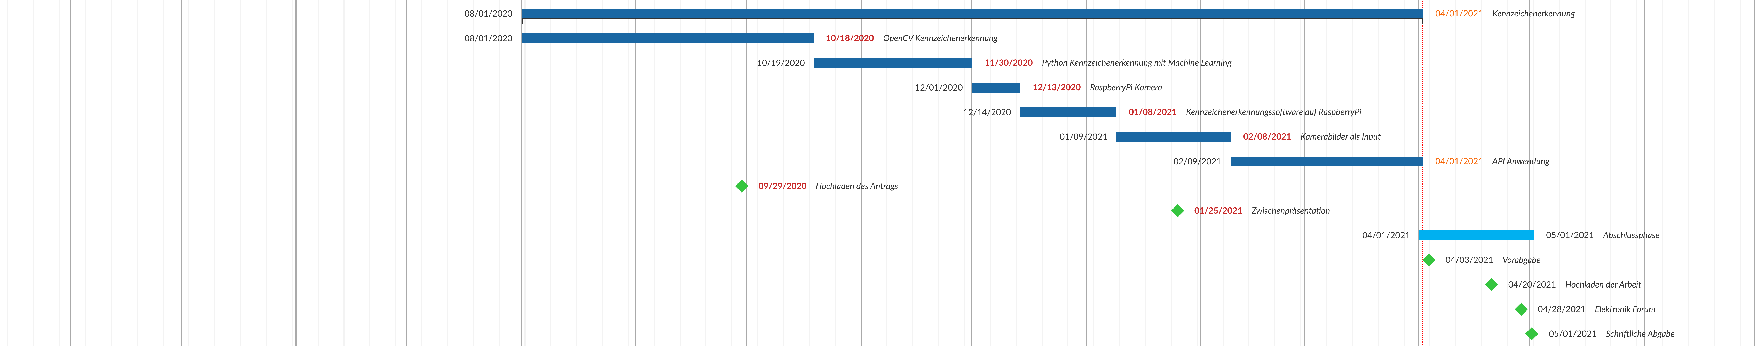
\includegraphics[width=1\linewidth]{gantt_2.pdf}}
  \caption{Gantt-Chart Teil 22}
\end{sidewaysfigure}
\pagebreak


%\section{Rechtliches}
%\pagebreak


\section{Einleitung}
Das Ziel dieser Arbeit ist es, eine Vereinfachung von Parkplatzüberwachungen zu
erstellen, welche möglichst überall eingesetzt werden kann. Dazu wird die Arbeit
in drei individuelle Teile aufgeteilt, welche einfach miteinander verbunden
werden können, um so einen modularen Aufbau bereitzustellen. Im ersten Teil geht
es um die Erkennung der Kennzeichen von Fahrzeugen. Dies wird beim Betreten und
Verlassen des Parkplatzes eingesetzt, um, festzustellen welches Fahrzeug sich im
Moment auf dem Parkplatz befindet. Zudem können dadurch unerlaubte Fahrzeuge
entdeckt werden und anschließend mögliche Schritte eingeleitet werden. Im
zweiten Teil geht es um die Erkennung von Fahrzeugen in einer Parklücke. Dazu
wird eine Spule unter jeder Parklücke verwendet, mit welcher festgestellt werden
kann, ob sich im Moment dort ein Fahrzeug befindet. Dadurch kann festgestellt
werden, welche Parkplätze besetzt sind und im Falle von mehrstöckigen Parkhäusern
kann die Auslastung der einzelnen Etagen überwacht werden. Im dritten Teil geht
es dann noch um die Darstellung und Verwaltung dieser Daten. Dazu wird eine
Web-Applikation bereitgestellt, welche alle Daten übersichtlich darstellt und
für den Parkplatzbetreiber und den Kunden unterschiedliche Benutzeroberflächen
bietet. Zudem kann die Web-Applikation mit wenig Aufwand von jedem
Parkplatzbetreiber personalisiert werden, was vor allem für Firmen interessant
ist, wenn sie diese in ihr Intranet einbauen möchten. Die Verbindung dieser drei
Teile erfolgt über eine eigens dafür geschriebenen API, wodurch die Daten über
das Internet übertragen werden können.
\pagebreak


%\section{Projektantrag}
%\input{sections/9_projektantrag.tex}
%\pagebreak


\section{Kennzeichenerkennung}
\def \sectionauthors {Samuel Bleiner}
\subsection{Anforderungen}
\lipsum[1-5]
\subsection{Vorstudie}
\lipsum[1-5]
\pagebreak


\section{Fahrzeugerkennung}
\def \sectionauthors {Dennis Köb}
\subsection{Anforderungen}
Das Ziel der Fahrzeugerkennung ist es Fahrzeuge auf mehrere Parklücken eines Parkplatzes zu erkennen. Die daraus 
gewonnen Zustände sollen an das Webinterface übermittelt und an den jeweilige Parklücken über LEDs ausgegeben werden. 
\subsection{Vorstudie}

\subsection{Erkennung von Metallen über Spulen}
Grundsätzlich werden in der Realität häufig Spulen verwendet, welche unter dem Asphalt verbaut sind, um darüberliegende
Fahrzeuge zu detektieren. Als Messprinzip wird die Änderung des magnetischen Widerstands $R_{m}$ bei konstanter magnetischer Spannung $U_{m}$ und
daraus resultierende magnetischen Fluss $\phi$
Es gelten für diese Größen der folgende Zusammenhänge:

\begin{equation} \label{eq:phi}
    \Phi = \frac{U_{m}}{R_{m}}
\end{equation}

Wobei \\
$\Phi$ = magnetischer Fluss \\
$R_{m}$ = magnetischer Widerstand \\
$U_{m}$ = magnetische Spannung
\pagebreak

Der magnetische Widerstand lässt sich wiederum durch die Eigneschaften der Spule bestimmen. Die Formel hierfür lautet:

\begin{equation} \label{eq:Rm}
    R_{m} = \frac{N \cdot (2a + 2b)}{\mu_{0} \cdot \mu_{r} \cdot A} 
\end{equation}


Wobei \\
\begin{equation} \label{eq:A}
    A = a \cdot b
\end{equation}
$N$ = Anzahl der Windungen der Spule \\
$a$ = Breite der Spule in m \\
$b$ = Länge der Spule in m\\
$\mu_{0}$ = \SI[per-mode = symbol]{1.2566e-6}{\newton\per\ampere\squared} = magnetische Feldkonstante \\
$\mu_{r}$ = relative Permeabilität  \\
$A$ = Fläche der Spule

Bis auf die relative Permeabilität sind alle alle anderen Variablen konstant. Daraus lässt sich schlussfolgern, dass der magnetische
Fluss $\Phi$ anhand der Gleichung \ref{eq:phi} und \ref{eq:Rm} proportional zur relativen Permeabilität ist. 

\begin{equation} \label{iq:phi}
    \Phi \propto \mu_{r}
\end{equation}
Der Fluss $\Phi$ hängt somit auch von den Materialien ab durch die er fließt. In der nächsten Abbildung kann man erkennen,
wie ein Fahrzeug über eine im Boden installierte Spule den magnetischen Fluss $\Phi$ und somit die magnetische Flussdichte $B$
beeinflussen kann. 

\begin{figure}[H]
    \centering
    \includegraphics[width=1\linewidth]{fahrzeugerkennung/Spuleninstallation.pdf}
    \caption{Installation der Spule}
  \end{figure}
Um diese Größen auslesbar zu machen, müssen diese magnetischen bei einer direkten Messung in elektrische Größen umgewandelt
werden.
Hierfür gelten folgende Zusammenhänge:

\begin{equation} \label{eq:L_phi}
    L = \frac{N \cdot \Phi}{I} = \frac{\Psi}{I} 
\end{equation}
Wobei \\
$L$ = Induktivität der Spule \\
$I$ = Strom der durch die Spule fließt \\
$N$ = Anzahl der Windungen der Spule \\
$\Psi$ = Verkettete Fluss

\pagebreak
\begin{equation} \label{eq:L_i}
    u(t) = L \cdot \frac{di(t)}{dt}
\end{equation}

Wobei \\
$L$ = Induktivität der Spule \\
$i(t)$ = Strom der durch die Spule fließt zum Zeitpunkt t \\
$u(t)$ = Spannung die an der Spule anliegt zum Zeitpunkt t \\
$t$ = Zeit in s \\
So lässt sich bei Bekanntheit von Strom und Spannung auf die Induktivität und mit der Gleichung \ref{eq:L_phi} 
und mit den Zusammenhang \ref{iq:phi} auf die magnetischen Eigenschaften des Materials rückschließen. 
Diese Art der Detektion bietet viele praktische Vorteile.

\begin{itemize}
    \item \textbf{Größerer Messbereich} \\
    Im Vergleich zu anderen Detektionsmethoden wie einer Leichtschranke kann man einen größeren Bereich durch die Wirkfläche
    der Spule abdecken. So lassen sich auch kleinere Kraftfahrzeuge wie Motorräder oder Mopeds besser erkennen.
    \item \textbf{Schutz vor Umweltfaktoren} \\
    Durch den Verbau im Boden ist die Messeinrichtung vor Umwelteinflüssen wie Regen, Frost, hohen beziehungsweise
    niedrigen Temperaturen und Korrosion besser geschütz. Dies verringert auch den Einfluss dieser Störfaktoren auf die Eigenschaften
    Spule und somit auf die daraus resultierenden Messergebnisse.
    \item \textbf{Ausschließung von Materialien} \\
    Alle nicht metallische Stoffe werden von diesem Messprinzip nicht wahrgenommen. So können Verschmutzungen wie Blätter und Staub, welche
    visuelle Sensoren stören können, die Detektion nicht behindern.
    
\end{itemize}
\subsubsection{Messung ferromagnetischer Metalle}
Um diese Dtektionsverfahren zu verstehen muss zuerst der Zusammenhang zwischen Induktivität und relativer Permeabilität verstanden werden.
Aus den Gleichungen \ref{eq:Rm}, \ref{eq:phi} und \ref{eq:L_phi} kann die folgende Proportionalität ermittelt werden:
\begin{equation} \label{iq:L_mu}
    L \propto \mu_{r}
\end{equation}
Bei ferromagnetischen Stoffen wie Eisen ist die relative Permeabilität sehr viel größer als 1. Wenn nun ein Auto oder 
eine anderes Vehikel sehr viel Eisen beinhaltet wirkt sich die dies steigernd auf die Induktivität der Spule aus. Die folgenden
Verfahren nutzen dieses Prinzip um die Belegung einer Parklücke zu bestimmen.

\paragraph{RL-Oszillator mit Timer Baustein}\mbox{}\\
Bei diesem Messverfahren wird die Änderung der Induktivität $L$ über die Änderung einer Stromladekurve über einen Widerstand
$R$ ermittelt. Eine Simulation in LTSPice mit folgendem Schaltbild kann die Auswirkung auf eine Ladekurve bei gleicher Spannung
und gleichem Widerstand gut darstellen.
\begin{figure}[H]
    \centering
    \includegraphics[width=1\linewidth]{fahrzeugerkennung/Ladekurven.png}
    \caption{LTSPice Blockbild zweier RL-Glieder}
\end{figure}
\pagebreak
Die daraus Resultierende Simulation im Zeitbereich ergibt folgendes Ergebnis:
hmm

\begin{figure}[H]
    \centering
    \includegraphics[width=1\linewidth]{fahrzeugerkennung/Ladekurven_ZB.png}
    \caption{Stromkurven zweier RL-Glieder}
\end{figure}

Es ist aus der letzten Abbildung erkennbar, dass sich eine größere Induktivität verlangsamend auf die Zunahme des Stromes auswirkt. Für Einschaltvorgänge kann diese Stromkurve
für RL-Glieder folgendermaßen beschrieben werden.

\begin{equation} \label{eq:i_L}
    i(t) = \frac{U_{0}}{R} \cdot (1 - e^{-\frac{t}{\tau}})
\end{equation}

\begin{equation} \label{eq:tau_RL}
    \tau = \frac{L}{R}
\end{equation} 

Wobei \\
$i(t)$ = Strom der durch die Spule fließt zum Zeitpunkt t \\
$L$ = Induktivität der Spule in H\\
$R$ = Widerstand in $\Omega$ \\
$U_0$ = Spannung die nach dem einschalten anliegt in V\\
$t$ = Zeit in s \\
$\tau$ = Zeitkonstante in $\frac{1}{s}$\\

Timer Bausteine wie der NE555 nutzen diese solche Verlaufskurven wenn sie als astabile Kippstufe konfiguriert sind.
Es gibt einen Eingang dieses Baustein meist CV für Control Voltage der die Spannung überwacht. Überschreitet diese Spannung zweit drittel
der Betriebsspannung schaltet er einen weiteren Pin, meist DIS für Discharge, auf 0V beziehungsweise auf Masse. Unterschreitet jedoch 
die Spannung am CV Pin ein drittel der Betriebsspannung so wird der DIS Pin auf Betriebsspannung geschalten. Diese beiden Pins 
sind über RC- oder RL- Glieder verbunden. Es entsteht somit ein Oszillator, welcher die Spannung am DIS Pin anhebt und absenkt.
Der NE555 kann dieses Signal über einen internen Komparator in ein Rechtecksignal umwandeln, welches besser von Mikrokontrollern ausgelesen
werden kann. Der Mikrokontroller kann so die Anzahl der ein einkommenden Takte über einen gewissen Zeitraum zählen und daraus eine Oszillatorfrequenz errechnen.
Die Zeitsignale lassen sich in LTSPice mit dem NE555 als Timer-Baustein simulieren.

\begin{figure}[H]
    \centering
    \includegraphics[width=0.6\linewidth]{fahrzeugerkennung/RL_Oszillator.png}
    \caption{RL-Oszillator mit NE555}
\end{figure}

\begin{figure}[H]
    \centering
    \includegraphics[width=1\linewidth]{fahrzeugerkennung/RL_Oszillator_ZB.png}
    \caption{RL-Oszillator mit NE555 Zeitsignale}
\end{figure}

Im oberen Diagramm ist der Verlauf des Stromes durch die Spule zu erkennen der wie erwartet zu- und abnimmt. Im unteren Diagramm ist in 
schwarz die Betriebsspannung als Referenz in rot der CV Pin und in blau der DIS Pin des NE555. Das rote Signal wechselt zwischen zwei drittel der Betriebsspannung 
und einem drittel der Betriebsspannung mit einer Frequenz von $f = \SI{438}{\kilo\hertz}$ bei einer Induktivität von $L = \SI{300}{\micro\henry}$, einem Widerstand $R4 = 100\Omega$ und einem
Widerstand $R5 = 300\Omega$. Die Simulation entspricht hier der Theorie, jedoch bricht das blaue Signal am PIN DIS in der Einschaltphase ein.
Der grund dafür ist der interne Widerstand des NE555, der ab einem gewissen Stromverbrauch für einen Spannungsabfall sorgt. Da es meist besser ist mit
niedrigen Frequenzen zu arbeiten ist es nach den Gleichungen \ref{eq:i_L} und \ref{eq:tau_RL} entweder nötig die Induktivität zu erhöhen oder die Widerstände zu verkleinern.
Die Induktivität lässt sich aber entweder durch erhöhen der Windungen oder durch Vergrößerung der Spule erreichen, was in vielen Fällen nicht möglich ist oder zunehmends kostspielig ist.
Die Reduktion der Widerstände führt zu einer Zunahme des Stromes und der Verlustleistung, was auch unerwünscht ist.
Aus diesen Gründen ist der RL-Oszillator nur für hohe Frequenzen geeignet. In der nächsten Abbildung sieht man die Schaltung bei verschiedene Induktivität
nämlich bei $L2 = \SI{100}{\micro\henry}$ und bei $L2 = \SI{1}{\milli\henry}$

\begin{figure}[H]
    \centering
    \includegraphics[width=1\linewidth]{fahrzeugerkennung/RL_Oszillator_vergleich2_ZB.png}
    \caption{Vergleich des NE555-Oszillators bei unterschiedlichen L}
\end{figure}

Eine Verzehnfachung der Induktivität führt zu einer Reduktion der Oszillatorfrequenz um den Faktor 10.

\begin{equation} \label{iq:f_NE555}
    f \propto \frac{1}{L}
\end{equation} 

\pagebreak
\subsubsection{Messung paramagnetischer Metalle}
Da nicht alle Metalle ferromagnetische Eigenschaften haben werden viele Stoffe wie Aluminium. Kupfer oder diverse Legierungen
von einer niederfrequenten Messung der Induktivität nicht wahrgenommen. Ein Effekt, welcher bei elektrischen Leitern abhilfe schaffen kann, sind 
die Eddy Currents. Wenn in einem Leiter ein magnetischen Feld einwirkt erzeugt dieses im Objekt Ströme, die wiederum ihr eigenes magnetische Feld erzeugen.
Die fließenden Ströme erzeugen im Objekt Ohmsche Verluste, welche normalerweise unerwünscht sind. Sie wirken auch einer Änderung der magnetischen Feldes entgegen,
da sie selbst Energie brauchen um ihre Richtung zu ändern. Je größer die Frequenz der eingespeisten Felddichte $B$ desto stärker wirkt die 
Flussdichte $B_{eddy}$ senkend auf die Gesamtflussdichte und so auf den magnetischen Fluss $\Phi$. 
Nach der Gleichung \ref{eq:L_phi} reduziert sich danach die Induktivität mit zunehmender Frequenz.


\begin{figure}[H]
    \centering
    \includegraphics[width=0.6\linewidth]{fahrzeugerkennung/Eddy_Currents.pdf}
    \caption{Eddy Currents in einem Leiter}
\end{figure}

Bei sehr hohen Frequenzen ist jedoch zu beachten, dass der Skin-Effekt die Querschnittsfläche, durch die der Wechselstrom fließen kann,
reduziert. Somit nimmt der Effekt der Eddy-Currents ab. Diese Phänomene werden jedoch nicht in dieser Arbeit behandelt, da sie außerhalb des Rahmens der 
Fahrzeugerkennung liegen. 

\paragraph{LC Oszillatoren}\mbox{}\\

Im Vergleich zum RL-Oszillator, der über eine astabile Kippstufe lauft, kann ein LC Oszillator seine Resonanzfrequenz nur durch das verstellen der Induktivität und der Kapazität 
eines Kondensators verändern. Zudem gibt es in der Theorie keine Wirkverluste, da die Energie abwechselnd zwischen magnetischer und elektroscher Energie umgewandelt wird. In der Realität gibt es jedoch
ohmsche Verluste, die zu einem Abklingen der Schwingung führen. Es braucht daher ein aktives Glied wie ein Transistor oder ein Operationsverstärker, der den Oszillator mit Energie versorgt.
\\
Der zeitliche Verlauf einer ungedämpften Schwingung kann in LTSPice simuliert werden indem wir eine Sprungfunktion auf ein LC Glied geben und einen Widerstand in Serie zum Kondensator oder zur
Spule geben.

\begin{figure}[H]
    \centering
    \includegraphics[width=0.6\linewidth]{fahrzeugerkennung/LC_Parallel.PNG}
    \caption{Parallelschwingkreis in LTSpice}
\end{figure}

\begin{figure}[H]
    \centering
    \includegraphics[width=1\linewidth]{fahrzeugerkennung/gedämpfte_schw.PNG}
    \caption{Gedämpfte Schwingung}
\end{figure}

Aus der Simulation ergibt sich über eine Cursormessung für die angegebenen Werte $L = \SI{100}{\milli\henry}$ und $C = \SI{100}{\milli\farad}$ eine Resonanzfrequenz einen Wert von $f = 15.85Hz$. Die Resonanzfrequenz für einfache LC-Schwingkreise lässt sich mit der
Thomsonschen Schwingungsgleichung errechnen:

\begin{equation} \label{eq:thomson}
    f = \frac{1}{2 \cdot \pi \sqrt{L \cdot C}}
\end{equation}

Wobei \\
$f$ = Resonanzfrequenz des LC-Gliedes\\
$L$ = Induktivität der Spule\\
$C$ = Kapazität des Kondensators\\

Wenn man die Werte $L = \SI{100}{\milli\henry}$ und $C = \SI{100}{\milli\farad}$ ind die Gleichung \ref{eq:thomson} einsetzt erhält man eine Resonanzfrequenz von $f = 15.915Hz$.
Allgemein tritt in LC-Glieder bei einer Phasenlage von $\varphi_{LC} = 180^{\circ}$ und bei der Frequenz nach der Thomsonschen Gleichung \ref{eq:thomson}  Resonanz auf. 

\paragraph{Einfluss von Induktivitätsänderungen auf LC-Oszillatoren}\mbox{}\\

Für die Fahrzeugerkennung ist es von Relevanz zu wissen wie die Frequenz dieser Oszillatoren auf die Änderung der Induktivität der im Boden verbauten Spule reagiert.
Wenn eine Parklücke frei ist besitzt die Spule eine Induktivität von $L_{0}$ und hat nach der Thomsonschen Gleichung \ref{eq:thomson} eine Resonanzfrequenz $f_{0}$. Für kleine Änderungen $\Delta L$ kann eine Näherung
der Frequenzänderung gemacht werden indem man in den Punkt $(f_{0}, L_{0})$ in den Graphen der Thomsonschen Gleichung aufgetragen über die Induktivität $L$ eine Tangente in diesen Punkt legt. Bei einer 
Kapazität von $C = \SI{1}{\micro\farad}$ erhält man folgenden Graphen: 

\begin{center}
    \begin{tikzpicture}
        
        \begin{axis}[
                axis x line=middle, 
                axis y line=middle, 
                xlabel={$L \text{ in } \si[]{\henry}$}, 
                ylabel={$f \text{ in } \si[]{\hertz}$}, 
                x=15cm/0.001,    
                y=0.0003cm,    
                grid =both,
                minor x tick num=1,
                subtickwidth=0pt,
                xtick={0,0.0001,...,0.001}, 
                ytick={0,5000,...,30000}, 
                xmin=0,  
                xmax=0.0011,   
                ymin=0,  
                ymax=32000,  
                scale = 0.7 
        ]
        
        \addplot [blue, thick, samples at={0,0.000001,0.000005,0.00001,...,0.0002,0.0003,0.0004,...,0.002}] {1/(2*pi*sqrt(x*1e-6))};
        \addplot[mark=none, red, thick] coordinates {(0, 20000) (0.4e-3, 0.1e4)};
        \addplot[mark=none, black, dashed] coordinates {(0, 1.4e4) (0.13e-3, 1.4e4)};
        \addplot[mark=none, black, dashed] coordinates {(0.13e-3, 0) (0.13e-3, 1.4e4)};
        \node[label={45:{($f_{0}$,$L_{0}$)}},circle,fill,inner sep=2pt] at (axis cs:0.13e-3,1.4e4) {};
        \node[label={45:{$L_{0}$}},circle,fill,inner sep=2pt] at (axis cs:0.13e-3,0) {};
        \node[label={45:{$f_{0}$}},circle,fill,inner sep=2pt] at (axis cs:0,1.4e4) {};
    \end{axis}
    \end{tikzpicture}
\end{center}

Mit dieser Näherung kann man mit des Differentials der Thomsonschen Gleichung \ref{eq:thomson} die Änderung des Funktionswertes $f(L \pm \Delta L) = \Delta f \approx df$ 
\begin{align*} \label{eq:df_L}
    df = \frac{\partial f}{\partial L}\bigg|_{L_{0}} \cdot dL \\ 
    df = \frac{\partial}{\partial L}  \left (  \frac{1}{2 \pi \sqrt{L_{0}C}} \right ) \Delta dL \\
    df = - \frac{1}{4 \pi} (L_{0}C)^{-\frac{3}{2}} \cdot \Delta L
\end{align*}

Für relative Änderungen der Induktivität $\Delta L$ um den Wert $L_{0}$ gilt:

\begin{equation} \label{eq:f_df}
    \frac{df}{f_{0}} =  -\frac{1}{2C} \cdot \frac{\Delta L}{L_{0}}
\end{equation}

Das bedeutet, dass eine kleine relative Änderung der Inuktivität $\frac{\Delta L}{L_{0}}$ bei gleicher Kapazität $C$ für eine halb so große relative Änderung in der Frequenz führt. 
Dieser Ansatz gilt nur bei kleinen $\Delta L$.

\paragraph{Messung der Frequenz eines Colpitts-Oszillator}\mbox{}\\

Der Colpitts-Oszillator ist eine Variante des LC-Oszillator und wird in der Praxis oft mit einem aktiven Element betrieben. Im Vergleich zu einem einfachen LC-Glied besitzt dieser Oszillator
zwei Kondensatoren. Das Schaltbild sieht so aus:

\begin{figure}[H]
    \centering
    \includegraphics[width=0.3\linewidth]{fahrzeugerkennung/Colpitts_LC.PNG}
    \caption{Colpitts LC-Glied}
\end{figure}

Dieses LC-Glied wird als Rückkoppelglied eingesetzt und sorgt für die nötige Phasendrehung von $\varphi_{LC} = 180^{\circ}$. Wie man in der obigen Abbildung sehen kann liegen die Kondensatoren 
$C_{1}$ und $C_{2}$ in Serie. Es ergibt sich daher eine Gesamtkapazität von $C_{ges}$.

\begin{equation} \label{eq:c_gescolpitts}
    C_{ges} = \frac{C_{1} \cdot C_{2}}{C_{1} + C_{2}}
\end{equation}
Durch einsetzen in die Thomsonsche Gleichung erhält man für die Resonanzfrequenz eines Colpitts-Oszillator:
\begin{equation} \label{eq:colpitts}
    f = \frac{1}{2 \cdot \pi \sqrt{L \cdot \left( \frac{C_{1} \cdot C_{2}}{C_{1} + C_{2}} \right) }}
\end{equation}

Wobei \\
$f$ = Resonanzfrequenz des Colpitts-Oszillator\\
$L$ = Induktivität der Spule\\
$C_{1}$ = Kapazität des Kondensators $C_{1}$\\
$C_{2}$ = Kapazität des Kondensators $C_{2}$\\

\pagebreak
Das aktive Element wird an die Anschlüsse der Spule angeschlossen muss selbst eine Phasendrehung von 180° liefern. Zusätzlich muss die Verstärkung des Gliedes größer als 1 damit eine dauerhafte 
Schwingung entstehen kann. Mit einem Operationsverstärker muss der nicht invertierende Eingang auf eine Bezugsspannung gelegt werden. Diese Bezugsspannung wird of in die Mitte des Versorgungsspannungsbereich
gelegt. Bei einem Spannungsbereich von $\SI{0}{\volt}$ bis $\SI{5}{\volt}$ ist eine Bezugsspannung von $\SI{2,5}{\volt}$ sinnvoll. Der invertierende Eingang wird an das Colpitts LC-Glied angeschlossen. Der Ausgang des Operationsverstärker wird über
einen Widerstand an das LC-Glied geschalten, damit das Rückkoppelglied besser vor übersteuerungen am Ausgang des Operationsverstärkers geschütz ist. 

\begin{figure}[H]
    \centering
    \includegraphics[width=0.4\linewidth]{fahrzeugerkennung/Colpitts_active.PNG}
    \caption{Aktiver Colpitts-Oszillator}
\end{figure}

Wenn man nun verschiedene Werte für Induktivität einsetzt ergibt sich durch die Simulation dieses Schaltbildes folgende Zeitsignale für den Ausgang des Operationsverstärker OUT und der Spannung SINE:

\begin{figure}[H]
    \centering
    \includegraphics[width=1\linewidth]{fahrzeugerkennung/Colpitts_active_ZB.PNG}
    \caption{Zeitsignale Colpitts-Oszillator}
\end{figure}

Es ist ersichtlich, dass dass eine Zunahme der Induktivität zu einer Abnahme in der Frequenz der beiden Signale führt.
\pagebreak
\subsection{RS485 Bussystem}
\subsubsection{Benutzte Standards}
\paragraph{ASCII}\mbox{}\\
ASCII ist eine amerkanischer Standard zur Kodierung einer 7 Bit langen folge. Dieser Standard ermöglicht es Zeichen wie 'A' oder 'b' sowie auch Zahlen und gewissen Sonderzeichen in Bits umzusetzen. 
\paragraph{USB}\mbox{}\\

Unter USB versteht man eine serielles Bussystem, welches dazu dient Peripherie Geräte an einen Computer zu verbinden. USB ermöglicht es Geräte während der Laufzeit des Betriebsssystems anzustecken und wieder zu entfernen.
Je nach Version des USB Standards ist es möglich unterschiedliche Datenraten und Leistungen zu verwenden, wobei neuere Standards Rückkompatibel zu alten Versionen sind. Für die Ansteeurng des Bussystems ist es notwendig einen Comupter anzuschließen. 
Der USB Standard bietet sich hier an, da er weit verbreitet ist und daher mit vielen Computern kompatibel ist.


\paragraph{UART}\mbox{}\\

Unter UART versteht man eine eine asynchrone serielle Schnittstelle. Die elektrische Schnittstelle braucht daher auch keine Taktleitung die dem Empfänger der Daten mitteilt wann er zu lesen hat. Stattdessen gibt es zwei Datenleitungen nämlich eine 
für das Senden TX und eine für das Lesen RX. Auf diesen Datenleitungen befinden sich nur die Bitströme des Empfängers und des Senders. Sie besitzen einen Ruhepegel von logisch 1.
UART synchronisiert sich idem es beim Start der Daten ein Startbit schickt, welche Sender und Empfänger synchronisiert. 
Diese beiden Geräte brauchen daher auch genaue interne Uhren um sich über den Zeitraum des Datenaustausches synchron zu halten.
Die Dauer diese Datenaustausches hängt vor allem von der Bitrate auch genannt Baudrate ab aber auch die Konfiguration der Anzahl von Datenbits und Paritätsbits haben Einfluss auf diese Größe. 
\\
In der folgenden Abbildung ist zeitliche Verlauf einer Datenleitung dargestellt es wird das Zeichen 'A' in ASCII codiert übertragen bei einer Baudrate von 57600 Zeichen pro Sekunde.

\begin{figure}[H]
    \centering
    \includegraphics[width=1\linewidth]{fahrzeugerkennung/UART_example.png}
    \caption{Beispiel einer UART Zeichenübertragung}
\end{figure}

\paragraph{RS485}\mbox{}\\

RS485 ist ein Standard für eine physikalische Schnittstelle für Datenübertragung von UART Daten. Er besitzt zwei symmetrische Leitung oft mit A und B bezeichnet, dessen Differenzspannung für die Auswertung
des Datenstromes herangezogen wird. Er ist dafür ausgelegt mehrere Geräte an die gleiche Leitungen anzuschließen. Die maximale Anzahl an Geräten ist mit 32 fix vorgegeben. Es ist zusätzlich notwendig die Spannungen 
$U_{A}$ und $U_{B}$ im Ruhezustand über einen IC oder einen Spannungsteiler auf fixe Potentiale zu legen. Der Spannungsteiler muss wie folgt aussehen um dem Standard zu entsprechen.

\begin{figure}[H]
    \centering
    \includegraphics[width=0.15\linewidth]{fahrzeugerkennung/RS485_bias.png}
    \caption{RS485 Widerstandsnetzwerk}
\end{figure}

Um diese physikalische Umwandlung zu ermöglichen ist eine Umwandlungs IC erforderlich. In dieser Arbeit wurde ausschließlich der MAX485CSA für Wandlung zwischen den Standardpegeln der UART
und die der RS485 Schnittstelle verwendet.

Dieser IC ist Bussfähig und kann daher seine Ausgänge hochohmig machen. Er besitzt folgende Eingänge und Ausgänge:
\begin{itemize}
    \item \textbf{!RE: Read enable} \\
    Wenn dieser Eingang auf logisch 0 gesetzt ist wertet der IC des Differenzsignal $U_{AB}$ aus und liefert des Ergebnis an den Ausgang RO.
    Ansonsten setzt er den Ausgang RO in den Tristate beziehungsweise auf hochohmig.
    \item \textbf{DE: Data enable} \\
    Wenn dieser Eingang auf logisch 1 gesetzt ist wird die Spannung am Eingang DI in die zugehörigen Pegel $U_{A}$ und $U_{B}$ umgewandelt.
    Ansonsten setzt er den Eingang DI in den Tristate beziehungsweise auf hochohmig.
    \item \textbf{RO: Read out} \\
    Ist die eingelesene Spannung die sich logisch aus der Differenzspannung $U_{AB}$ ergibt wenn !RE auf logisch 0 ist.
    \item \textbf{DI: Data In} \\
    Ist die eingehende Spannung die auf die RS485 Schnittstelle geschrieben werden soll, wenn der Eingang DE auf logisch 1 ist.
\end{itemize}

Die Auswertung der Differenzspannung $U_{AB}$ kann auch in der folgenden Tabelle aus dem Datenblatt des MAX485CSA entnommen werden. 

\begin{figure}[H]
    \centering
    \includegraphics[width=0.6\linewidth]{fahrzeugerkennung/RS485_receiving_table.png}
    \caption{Logische Tabelle für $U_{AB}$}
\end{figure}

In der folgenden Abbildung wird wieder an 'A' ASCII kodiert versendet nur dieses mal wird eine RS485 Schnittstelle mit den entsprechenden Pegeln verwendet verwendet.
In blau ist die Spannung $U_{A}$ und in orange die Spannung $U_{B}$ zu sehen. Darunter befindet sich das logische UART Signal am Ausgang RO. 

\begin{figure}[H]
    \centering
    \includegraphics[width=1\linewidth]{fahrzeugerkennung/RS485_example.png}
    \caption{Beispiel einer RS485 Zeichenübertragung}
\end{figure}

\paragraph{RJ45}\mbox{}\\
Um die Anzahl der Kabel zu minimieren und um das Anschließen von Geräten an den Bus einfach zu halten ist ein
mehradriger Stecker mit zugehörigem Kabel nötig.\\
Der RJ-45 Stecker ist eine genormter Stecker und besitzt insgesamt 8 Adern und ist für Kommunikationsanschlüsse gedacht. Er kann daher größere Datenraten zulassen und viele auf dem
Markt vorhandene Kabel haben zusätzliche Abschirmungen, die die Datenleitungen vor elektrischen Störungen schützen. 

\begin{figure}[H]
    \centering
    \includegraphics[width=0.6\linewidth]{fahrzeugerkennung/RJ45_connectors.jpg}
    \caption{RJ45 Steckerbuchse und Kabel}
\end{figure}



\subsubsection{Aufbau}

Das Bussystem wir über eine Master Slave Struktur verwaltet was heißt das nur das ein einzelnes Master-Gerät als erstes andere Teilnehmer am Bus ansprechen kann.
Slave-Geräte können nur nach Anfrage des Masters auf den Bus schreiben. Neben der Steuerung der Kommunikation sollte das Master-Gerät aus praktischen Gründen ebenfalls die Slave-Geräte
mit Energie versorgen und ihnen eindeutige Adressen zuweisen können. \\

In den unteren Abbildungen sind der logische Aufbau und der physikalische Aufbau zu sehen.
Auf die einzelnen Funktionen diverser Leitungen wird in den folgenden Paragraphen eingegangen.

\begin{figure}[H]
    \centering
    \includegraphics[width=1\linewidth]{fahrzeugerkennung/übersicht_bus.pdf}
    \caption{Logische Übersicht des Bussystems}
\end{figure}

\begin{figure}[H]
    \centering
    \includegraphics[width=1\linewidth]{fahrzeugerkennung/übersicht_irl.jpg}
    \caption{Physische Übersicht des Bussystems}
\end{figure}

Die elektrische Belegung der Leitungen ist wie in der folgenden Tabelle festgelegt worden. Mit dieser Belegung ist es möglich die Slave-Geräte an den RS485 Datenbus zu legen,
sie mit Spannung zu versorgen und die Adressvergabe mit einer zusätzlichen Logikleitung zu regeln. 

\begin{table}[]
    \centering
    \begin{tabular}{|c|c|c|c|}
        \hline
        \textbf{Pinnummer} & \textbf{Farbe} & \textbf{Netz} & \textbf{Beschreibung}                      \\ \hline
        1                  & Orange / weiß  & GND           & Masse                                      \\ \hline
        2                  & Orange         & +5V           & 5 Volt Versorgungsspannung                 \\ \hline
        3                  & Grün / weiß    &               & unbelegt                                   \\ \hline
        4                  & Blau           & A             & RS485 positives Datensignal                \\ \hline
        5                  & Blau / weiß    & B             & RS485 negatives Datensignal                \\ \hline
        6                  & Grün           & VCC           & Positive Versorgungsspannung +9V bis 30V   \\ \hline
        7                  & Braun / weiß   & GND           & Masse                                      \\ \hline
        8                  & Braun          & ADR           & Logiksignal zur Vergabe der Slave Adressen \\ \hline
    \end{tabular}
    \caption{RJ45 allgemeine Pinbelegung}
\end{table}

\paragraph{Funktion der Adresslogikleitung}\mbox{}\\

Da alle Teilnehmer des RS485-Busses parallel an den Datenleitung A und B liegen kann der Master sie voneinander nicht unterscheiden. Dieses Probleme beseitigt die Adressleitung, welche
die einzelnen Geräte logisch aneinanderreiht.

\begin{figure}[H]
    \centering
    \includegraphics[width=1\linewidth]{fahrzeugerkennung/adress_function.pdf}
    \caption{Anordnung der Slave-Geräte mit Adresslogikleitung}
\end{figure}

Jedes Slave-Gerät setzt seine Adresslogikleitung über einen Pullup-Widerstand auf logisch 1 wenn es keine Adresse zugeordnet bekommen hat.
Als erstes in der Reihe ist der Master, der seine Adresslogikleitung auf logisch 0 setzt und so dem ersten Gerät in der Kette bekannt gibt, dass es eine Adresse zugewiesen bekommt. Wenn es
diese Adresse bekommen hat legt das Slave-Gerät seine ausgehende Adresslogikleitung ADRO auf logisch 0. So kann das nächste Gerät in der Kette erkennen, dass es eine Adresse zugewiesen kriegt, 
indem es auf die eingehende Adressleitung ADRI achtet.\\
In den folgenden Abbildungwn sieht man wie die Geräte über den RJ45 Stecker elektrisch am Bus hängen. Der Master hat nur einen Stecker und hat seine Adresslogikleitung fix auf logisch 0 gelegt.
Die Slaves hingegen brauchen zwei Stecker um die Adresskette zu bilden und unterscheiden zwischen eingehender Adresslogikleitung ADRI und ausgehender Adresslogikleitung ADRO. \\
Wenn jedoch die Slaves falsche herum angeschlossen werden und ADRI und ADRO vertauscht sind kann dieser Fehler vom Mikrokontroller erkannt und behoben werden. Die genauen Details dieser Funktion 
werden in späteren Abschnitten erklärt. 

\begin{figure}[H]
    \centering
    \includegraphics[width=0.6\linewidth]{fahrzeugerkennung/RJ45_slave.png}
    \caption{RJ45 Pinbelegung des Slave-Geräts}
\end{figure}

\begin{figure}[H]
    \centering
    \includegraphics[width=0.3\linewidth]{fahrzeugerkennung/RJ45_master.png}
    \caption{RJ45 Pinbelegung des Master-USB-Geräts}
\end{figure}

\paragraph{Versorgungsleitungen VCC und GND}\mbox{}\\

Da es für jeden Parkplatz ein Slave-Gerät gibt ist die Länge der Busleitung nicht unbeträchtlich. Es kann so entlang der Leitung zu abfällen in der Versorgungsspannung aufgrund des Widerstands der langen Leitung.
Um dem entgegenzuwirken muss die Versorgungsspannung VCC bezogen auf Masse größer als die benötigte Spannung an den Geräten sein. Die Slave-Geräte besitzen alle einen Linearregler der für einen konstante Spannung von 5V sorgt.
Die Eingangsspannung des Spannungsreglers muss je nach Ausführung um eine gewisse Differenzspannung größer sein als die am Ausgang benötigte Spannung sein. Dieser Wert wird als \textit{Dropout Voltage} bezeichnet. 
Für den IC L78L05ACD lässt sich aus dem Datenblatt folgende Spannung nachlesen: $\SI{2}{\volt}$

\begin{figure}[H]
    \centering
    \includegraphics[width=1\linewidth]{fahrzeugerkennung/L78L05_characteristics.png}
    \caption{Elektrische Eigenschaften des L78L05ACD}
\end{figure}

Daraus lasst sich schließen dass der IC mindestens eine Spannung von $\SI{7}{\volt}$ braucht um zu funktionieren. Als Eingangsspannung für alle Messung wurde $\SI{9}{\volt}$ verwendet. Nach Datenblatt ist die Eingangsspannung auf 
einen Maximalwert von $\SI{30}{\volt}$ beschränkt. Es ist zu beachten, dass eine Erhöhung der Eingangsspannung zu mehr Verlusten am Linearregler führt und somit für eine schlechte Effizienz sorgt.

\subsubsection{Implementation eines eigenen Protokolls}

\subsection{Mikrokontroller Slave-Geräte}
\subsubsection{Überblick}
\subsubsection{Atmega328PB}
\subsubsection{Peripherie des Mikrokontrollers}
\paragraph{Spannungswandler}
\paragraph{RS485 Pegelwandler}
\paragraph{Digitale Ein- und Ausgänge}
\subsubsection{Layout des Slave-Gerätes}
\subsubsection{Gehäuse}


\subsection{USB-Master}
\subsubsection{USB-Bussadapter Gerät}
\paragraph{Überblick}
\paragraph{FT232RL}
\paragraph{Spannungsversorgung}
\paragraph{USB-C Anschluss}
\paragraph{Layout des Master-Geräts}
\paragraph{Gehäuse}

\subsubsection{Master Programm}
\paragraph{Benötigte Software}
\paragraph{Adressvergabe}
\paragraph{Frequenzauslesung}

\paragraph{Auswertung}
\paragraph{API-Post}

\subsubsection{RaspberryPi als Mastergerät}
\paragraph{SSH Remote Zugriff}
\paragraph{Code Deployment}
\paragraph{Unittest}

\pagebreak



\pagebreak


\section{Webinterface}
\def \sectionauthors {Philipp Kraft}

\subsection{Einleitung}

\subsection{Anforderungen}
Das Webinterface hat auf der einen Seite die Aufgabe die Kommunikation mit der
Kennzeichenerkennung und der Fahrzeugerkennung sicherzustellen und auf der
anderen Seite die Verwaltung und Darstellung der gewonnen Daten.

\subsection{Verwendete Technologien}
\subsubsection{HTML}
\acs*{HTML} steht hierbei für \acl*{HTML} und ist eine Auszeichnungssprache
welche vom \ac*{W3C}\footnote{\url{https://www.w3.org} } entwickelt wird. \ac*{HTML} ist
De-Facto-Standard um Inhalte in Browsern darzustellen. \acs*{HTML} ist dabei aber
nicht für die visuelle Darstellung verantwortlich sondern nur für die
semantische Struktur. Der Sinn dahinter ist, dass der Inhalt und die Vorgaben an
die Darstellung möglichst gut getrennt ist. Für die Formatierung kommt die Stylesheet-Sprache \ac*{CSS} zum Einsatz,
welche ebenfalls vom \acl*{W3C} entwickelt wird. Die aktuellste Version der
\acs*{HTML} Spezifikation ist
HTML5\footnote{\url{https://www.w3.org/2014/10/html5-rec.html.en}} und wurde am
28. Oktober 2014 vom \acs*{W3C} vorgelegt.

\paragraph{Beispielhafte HTML Seite}\mbox{}\\
Eine \acs*{HTML} Seite setzt sich aus einer Vielzahl von sogenannten Elementen
zusammen. Ein Element besteht aus einem Start Tag und aus einem End Tag, der
Inhalt wird zwischen diese Tags geschrieben. Nun folgt eine einfache HTML Seite,
welche die Grundlegenden Funktionen von HTML und CSS darlegen soll.

\begin{listing}[H]
  \begin{minted}{html}
    <!DOCTYPE html>
    <html>
    <head>
    <title>Titel</title>ü
    </head>
    <body>

    <h1>Überschrift</h1>
    <p>Paragraph</p>

    </body>
    </html>
  \end{minted}
  \caption{index.html}
  \label{lst:simple_html_site}
\end{listing}

Das Element \verb|<!DOCTYPE html>| deklariert, dass die folgende Seite den HTML5
Standard verwendet. Danach folgt mit \verb|<html>| das Wurzelelement, dass alle
anderen Elemente beinhaltet. Das \verb|<head>| Element beinhaltet verschiedene
Metadaten d.h. Daten die nicht angezeigt werden. Im oben gezeigten Beispiel
Code~\ref{lst:simple_html_site} wird nur der Title des Dokuments gesetzt, dieser
wird im Browser Tab angezeigt. Es können aber auch noch andere Daten gesetzt
bzw. eingebunden werden:

\begin{itemize}
  \item Character Set
  \item Styles
  \item Scripts
  \item Viewport
  \item Sonstige Metainformationen (Author, Keywords)
\end{itemize}

\begin{figure}[H]
  \centering
  \includegraphics[width=1\linewidth]{webinterface/simple_html_site.png}
  \caption{Einfache HTML Seite}
\end{figure}

\subsubsection{CSS}
Wie bereits angesprochen ist \ac*{CSS} für die Formatierung bzw. die visuelle
Darstellung der einzelnen HTML-Elemente verantwortlich. Der Standard wird wie
bei HTML vom \acs*{W3C} spezifiziert und die aktuellste Version ist CSS3 was so
viel bedeutet wie \acs*{CSS} Level 3, wobei nur einzelne Teile als Empfehlung
durch das \acs*{W3C} vorgelegt wurden, beispielweise das CSS Color Module Level
3\footnote{\url{https://www.w3.org/TR/css-color-3}}. Um die Funktion
darzustellen wird die vorherige HTML Seite nun mit CSS ergänzt.

\begin{listing}[H]
  \begin{minted}{css}
    body {
      background-color: deepskyblue;
    }

    h1 {
      color: white;
      text-align: center;
      font-family: verdana;
    }

    p {
      color: wheat;
      font-family: verdana;
      font-size: 20px;
    }
  \end{minted}
  \caption{style.css}
\end{listing}

Nun muss dieses Stylesheet nur noch im \verb|<head>| Tag mit\\
\mintinline{css}{  <link rel="stylesheet" href="style.css">} eingebunden
werden.

\begin{figure}[H]
  \centering
  \includegraphics[width=1\linewidth]{webinterface/simple_html_site_with_css.png}
  \caption{Einfache HTML Seite mit CSS}
\end{figure}

Es lässt sich nun deutlich erkennen, dass sich die Webseite stark verändert hat
von den Farben bis zu der Schriftart. HTML und CSS bieten noch viel mehr
Funktionen, eine Vielzahl der Funktionen sind auf der Website
w3schools\footnote{\url{https://www.w3schools.com/html} und
\url{https://www.w3schools.com/css}} zu finden.

\subsubsection{JavaScript}
Es folgt nun eine weitere sehr wichtige Technologie und die meist verwendete
Programmiersprache überhaupt laut der Stack Overflow Developer Survey
2020\footnote{\url{https://insights.stackoverflow.com/survey/2020}}. \ac*{JS}
ermöglicht es dynamische Webseiten zu erstellen, dabei wird der Code direkt
lokal im Browser ausgeführt. Jedoch ist JavaScript nicht mehr nur auf das
Frontend\footnote{Grafische Benutzeroberfläche mit der der Benutzer interagiert}
mehr beschränkt, es möglich mit Frameworks wie Node.js auch
Backend\footnote{Verarbeitung von Daten auf beispielsweise einem Server}
Applikationen zu schreiben und somit ist es möglich Full-Stack\footnote{Front-
und Backend}-Anwendungen vollständig mit
\acl*{JS} zu entwickeln. Eine der wichtigsten Anwendungsgebiete ist die
Manipulation von Elementen über das \ac*{DOM}. Der Standards wird unter dem
Namen ECMA Script von der Organisation Ecma
International\footnote{\url{https://www.ecma-international.org}}
veröffentlicht und die aktuellste Version ist
\textbf{ECMA-262}.

\subsubsection{PHP}
\ac*{PHP} ist eine Skriptsprache um dynamische Webseiten zu realisieren, jedoch
wird nicht wie bei \acl*{JS} der Code auf dem Client ausgeführt sondern auf dem
Server, dort wird die HTML-Ausgabe generiert und dem Client zugesendet.
Somit ist es nicht möglich den Code als Benutzer zu betrachten. Grundsätzlich
ist PHP als synchrone Sprache geplant worden, es ist jedoch auch möglich
asynchron zu Programmieren um die Performance zu steigern. Die aktuellste
Version ist \acs*{PHP} 8\footnote{\url{https://www.php.net/docs.php}}.


\subsubsection{TailwindCSS}
Es gibt eine Vielzahl von CSS-Frameworks, das Ziel ist ein einfacheres und
schnelleres erstellen von Webseiten, dazu gehören neben TailwindCSS folgende
relevanten Frameworks.

\begin{itemize}
  \item Bootstrap (\url{https://getbootstrap.com})
  \item Foundation (\url{https://get.foundation})
  \item Materialize (\url{https://materializecss.com})
\end{itemize}

Viele von diesen CSS Frameworks verwenden vorgefertigte Components welche direkt
verwendet werden können, dies führt dazu, dass die Entwicklung sehr rasch ist.
Dort unterscheidet sich TailwindCSS von den anderen CSS Frameworks, dort
existieren sogenannte Utility-Classes, diese können direkt im \acs*{HTML} auf die
einzelnen Elemente angewendet werden.

%\subsubsection{Vue}

\subsubsection{Laravel}
Laravel\footnote{\url{https://laravel.com/}} ist ein Open-Source PHP-Framework, es erleichtert die Entwicklung und
erhöht die Sicherheit und auch durch die zahlreichen First-Party-Packages bietet
Laravel ein sehr hochwertiges Ecosystem. Da Laravel ein sehr wichtiger Bestandteil des
Webinterfaces ist wird später noch genauer auf die einzelne Funktionen des
Frameworks eingegangen. Laravel wird seit Juni 2011 entwickelt und erhält
jährlich eine neue Version, aktuell ist Laravel 8 die neuste Version.\\

Das Framework folgt dem sogenannten \ac*{MVC} Muster das bedeutet, dass die
Programmierlogik in drei verschiedene Teile unterteilt wird. Der Sinn dahinter
ist, dass die Anwendung dadurch sehr flexibel ist und später leichter erweitert
werden kann oder einzelne Teile wiederverwendet werden können.

\begin{itemize}
  \item \textbf{Model} \\
  Hier befindet sich die Datenstruktur der Anwendung. In Laravel kann dies
  beispielsweise das Model \verb|User| sein.
  \item \textbf{View} \\
  In der View befindet sich die Präsentationsebene, im Fall von Laravel sind das
  Components und Layouts.
  \item \textbf{Controller} \\
  In den Controllern der Anwendung befindet sich die Logik um beispielsweise
  durch das Absenden eines Formulares einen Eintrag in der Datenbank zu erstellen. 
\end{itemize}

Laravel besitzt eine sehr ausführliche Dokumentation welche unter
(\url{https://laravel.com/docs/8.x}) zu erreichen ist.

\paragraph{Routing}\mbox{}\\
In Laravel erfolgt durch ein Routefile unter \verb|routes/web.php|. API Requests
haben ein eigenes Routefile unter \verb|routes/api.php| und erhalten einen
\verb|/api| Prefix. Diese Dateien werden dann automatisch durch einen Service
Provider von Laravel geladen.\\

Der Laravel Router erlaubt folgende HTTP-Anfragemethoden:
\begin{itemize}
  \item \textbf{GET} (Fordert Ressource an)\\
  \mintinline{php}{  Route::get($uri, $callback);}
  \item \textbf{POST} (Neue Ressource erstellen)\\
  \mintinline{php}{  Route::post($uri, $callback););}
  \item \textbf{PUT} (Ressource ersetzen oder erstellen)\\
  \mintinline{php}{  Route::put($uri, $callback);}
  \item \textbf{PATCH} (Ressource ändern)\\
  \mintinline{php}{  Route::patch($uri, $callback);}
  \item \textbf{DELETE} (Löscht Ressource)\\
  \mintinline{php}{  Route::delete($uri, $callback);}
  \item \textbf{OPTIONS} (Liste von unterstützen Methoden des Servers)\\
  \mintinline{php}{  Route::options($uri, $callback);}
\end{itemize}

Im folgenden Ausschnitt Code~\ref{lst:user_routes} werden ein Teil der Routen von den Benutzern dargelegt. Dabei lässt
sich erkennen, dass die Routen sich in einer Gruppe befinden, welche den Prefix
\verb|/admin| und die Middleware \verb|verified| hat das bedeutet, dass der Benutzer
eingeloggt sein muss um diese Routen aufzurufen. Dabei verweisen die Routen auf
einzelne Methoden im UserController. Schlussendlich werden mit der name-Methode
die Routen benannt, damit sie später im Code einfach referenziert werden können.

\begin{listing}[H]
  \begin{minted}{php}
    <?php
    Route::group(['middleware' => 'verified', 'prefix' => 'admin'], 
    function () {
      Route::get('users', [UserController::class, 'index'])->name('users.index');
      Route::get('users/create', [UserController::class, 'create'])->name('users.create');
      Route::post('users', [UserController::class, 'store'])->name('users.store');
    });
  \end{minted}
  \caption{web.php}
  \label{lst:user_routes}
\end{listing}

\paragraph{Blade Templates}\mbox{}\\
Blade ist eine Template Engine, die mit Laravel mitgeliefert wird. Blade
erleichtert und vereinfacht das Verwenden von PHP Code in HTML, dabei wird der
Blade Syntax in normalen PHP Code compiliert. Blade Dateien werden mit der
Extension \verb|.blade.php| erstellt. Damit der Inhalt der einzelnen Seiten
dynamisch ist müssen Daten übergeben werden, dies erfolgt über die Controller.\\

Um nun Inhalt innerhalb eines Blade Files anzuzeigen verwendet Blade doppelt
Geschweifte Klammern.

\begin{listing}[H]
  \begin{minted}{php}
    Hallo, {{ $user->full_name }}.
  \end{minted}
  \caption{example.blade.php}
  \label{lst:blade_example}
\end{listing}

Im Code~\ref{lst:blade_example} wird nun auf das übergebene Model \verb|User|
zugegriffen und der Name ausgegeben.

\paragraph{Controllers}\mbox{}\\
Es besteht theoretisch die Möglichkeit die komplette Logik für die bearbeitung
von Anfragen direkt in den Route Files zu platzieren, dies ist jedoch sehr
unübersichtlich und deshalb ist es sinnvoll diese Logik in Controller Klassen
auszulagern. Dabei werden ähnliche Anfragen zusammengeführt, so ist es sinnvoll
alle Anfragen wie in Code~\ref{lst:user_routes} im gleichen Controller
zusammenzuführen.

\begin{listing}[H]
  \begin{minted}{php}
    <?php
    namespace App\Http\Controllers;

    use Illuminate\Http\Request;
    use App\Models\User;
    use Illuminate\Support\Facades\Hash;
    use App\Http\Requests\StoreUser;
    use App\Http\Requests\UpdateUser;
    use App\Models\Role;
    use Image;

    class UserController extends Controller
    {
        public function index()
        {
            $this->authorize('index', User::class);
            $users = User::orderBy('id', 'asc')->paginate(25, ['*'], 'users');
            return view('users.index')->with('users', $users);
        }
    ...
  \end{minted}
  \caption{UserController.php}
\end{listing}

\paragraph{Artisan CLI}\mbox{}\\
Artisan ist ein Kommandozeilen Tool von Laravel und zentraler Bestandteil und
stellt eine Fülle an sehr nützlichen Befehlen dem Entwickler zur verfügung.
Mithilfe von Artisan können neue Controller, Models, Migrations und vieles sehr
einfach erstellt werden. Da es sehr viele Befehle gibt folgen hier nur die
wichtigstens Befehle:

\begin{itemize}
  \item \textbf{php artisan list}\\
  Zeigt eine Liste aller verfügbaren Befehle an
  \item \textbf{php artisan serve}\\
  Startet einen PHP Development Server unter dem Port 8000
  \item \textbf{php artisan make:model <name>}\\
  Erstellt ein neues Model
  \item \textbf{php artisan make:migration <name>}\\
  Erstellt ein neue Migrations
  \item \textbf{php artisan make:controller <name>}\\
  Erstellt ein neuer Controller
  \item \textbf{php artisan migrate}\\
  Führt die Datenbank Migration Files aus
\end{itemize}

\paragraph{Migrations}\mbox{}\\
Datenbank Migrations sind praktisch Vorlagen wie einzelne Tabellen in der Datenbank auszusehen
haben. Migrations erleichtern die Handhabung von SQL Datenbank im Team mithilfe
von Source Control wie Git um einiges.

\begin{listing}[H]
  \begin{minted}{php}
    <?php
    class CreateUsersTable extends Migration
    {
        public function up()
        {
            Schema::create('users', function (Blueprint $table) {
                $table->id();
                $table->string('first_name');
                $table->string('last_name');
                $table->string('email')->unique();
                $table->string('avatar')->default('default.png');
                $table->timestamp('email_verified_at')->nullable();
                $table->string('password');
                $table->string('last_login_ip')->nullable();
                $table->timestamp('last_login_at')->nullable();
                $table->rememberToken();
                $table->timestamps();
            });
        }
    
        public function down()
        {
            Schema::dropIfExists('users');
        }
    }
  \end{minted}
  \caption{create\_users\_table.php}
  \label{lst:create_users_table}
\end{listing}

Im Code~\ref{lst:create_users_table} sind zwei Methoden zu erkennen, \verb|up|
und \verb|down|, in der \verb|up| Methode werden neue Tabellen und Spalten in der
Datenbank erstellt, bei der \verb|down| Methode wird alles von der \verb|up| Methode
rückgängig gemacht, in diesem Fall wird die komplette Tabelle gelöscht. Um nun
die Datenbank zu migrieren muss in der Artisan \acs*{CLI} Befehl \verb|php artisan migrate|
ausgeführt werden, dabei werden alle Migrations im Verzeichnis
\verb|database/migrations| ausgeführt.

\paragraph{Eloquent ORM}\mbox{}\\
Eloquent ist ein \ac*{ORM} d.h. um auf die \acs*{SQL} Datenbank zuzugreifen müssen
keine Raw \acs*{SQL} Queries ausgeführt werden. Im Code erscheint die Datenbank als
objektorientierte Datenbank und erleichtert somit dem Umgang mit der Datenbank.
Dabei entspricht besitzt jede Tabelle in der Datenbank einem dazugehöriges Model,
dieses Model wird verwendet um im Code mit der Datenbank zu interagieren. Ein
weiter Vorteil ist, dass der Code sehr übersichtlich und leicht lesbar ist,
jedoch wird die Ausführungszeit leicht erhöht, was jedoch keine große Rolle bei
kleinen- bis mittelgroßen Webseiten spielt.

\begin{listing}[H]
  \begin{minted}{php}
    <?php
    User::where('first_name', 'Philipp')->first();
  \end{minted}
  \caption{Eloquent Query}
  \label{lst:eloquent_query}
\end{listing}

\begin{listing}[H]
  \begin{minted}{sql}
    SELECT * FROM `users` WHERE `first_name` = Philipp
  \end{minted}
  \caption{Raw SQL Query}
  \label{lst:raw_sql_query}
\end{listing}

Beim Vergleich zwischen dem Code~\ref{lst:eloquent_query} und
Code~\ref{lst:raw_sql_query} ist es erkenntlich, dass der Eloquent Query
verständlicher ist. Besonders bei komplexeren Queries ist Eloquent den RAW
\acs*{SQL} Queries im Bezug auf die Lesbarkeit stark überlegen.


\paragraph{Laravel Sanctum}\mbox{}\\
Laravel Sanctum ist ein First-Party-Package von den Entwicklern von Laravel und
ermöglicht eine einfache Authentifizierung mithilfe von API-Tokens. Dabei wird
der vom Benutzer erstellte API-Token im HTTP Header \verb|Authorization|
mitgeliefert und somit autorisiert. Da es sich hierbei um ein
Sicherheitskritisches Modul handelt ist es besonders wichtig, dass dieser Code
nahezu Fehlerfrei ist und dies wird durch kontinuierliche Updates und Patches garantiert.
 
%\paragraph{Laravel Mix}
%\paragraph{Sessions}
%\paragraph{Middleware}


\subsection{Lokale Entwicklungsumgebung mit Laragon}
Für die Programmierung des Webinterfaces müssen zuerst einige Vorkehrungen
getroffen werden, dazu zählt zu einem die Installation von benötigter Software
und deren konfiguration.


\subsubsection{Benötigte Software}

\begin{itemize}
  \item \textbf{Laragon} (\url{https://laragon.org}) \\Beinhaltet mehrere
        Softwarepakete die für die Entwicklung notwendig sind.
        \begin{itemize}
          \item Apache HTTP Server
          \item MySQL
          \item PHP
        \end{itemize}
  \item \textbf{phpMyAdmin} (\url{https://www.phpmyadmin.net}) \\ Webinterface
        für MySQL
  \item \textbf{Composer} (\url{https://getcomposer.org}) \\ Paketmanager für
        PHP
  \item \textbf{Git} (\url{https://git-scm.com}) \\ Versionskontrolle
  \item \textbf{Visual Studio Code} (\url{https://code.visualstudio.com}) \\
        Quelltext-Editor
\end{itemize}


\subsubsection{Konfiguration von PHP}
Um PHP Befehle von der Kommandozeile auszuführen muss die Installation zuerst in
den Windows Path Variables hinzugefügt werden.

Dies erfolgt durch die \verb|Advanced System Settings| $\blacktriangleright$
\verb|Environment Variables| $\blacktriangleright$ \verb|System Variables|.
Dort kann nun die Path Variable editiert werden und der Pfad hinzugefügt werden
in welchem die \verb|php.exe| liegt.

\begin{figure}[H]
  \centering
  \includegraphics[width=0.6\linewidth]{webinterface/advanced_system_settings.png}
  \caption{Advanced System Settings}
\end{figure}

\begin{figure}[H]
  \centering
  \includegraphics[width=0.6\linewidth]{webinterface/system_variables.png}
  \caption{System Variables}
\end{figure}

\begin{figure}[H]
  \centering
  \includegraphics[width=0.6\linewidth]{webinterface/environment_variable.png}
  \caption{Environment Variables}
\end{figure}

Die korrekte konfiguration kann durch die Kommandozeile geprüft werden, dort
muss das Befehl \verb|php -v| ausgeführt werden. Dabei ist zu beachten, dass
nach dem hinzufügen der Path Variable die gewählte Kommandozeile neu gestartet
werden muss.

\begin{figure}[H]
  \centering
  \includegraphics[width=1\linewidth]{webinterface/php_version.png}
  \caption{PHP Version}
\end{figure}

Somit ist PHP korrekt konfiguriert.


\subsubsection{Installation von phpMyAdmin}
phpMyAdmin ist ein Tool, welches den Umgang mit MySQL Datenbanken mit einem
Webinterface erleichtert. Die aktuellste Version lässt sich von
\url{https://www.phpmyadmin.net/downloads} downloaden. Dieses Archiv muss
entpackt werden und ausgehend vom Laragon Root Verzeichnis in das Verzeichnis
\verb|/etc/apps| kopiert werden. Um die Installation zu überprüfen muss der
Apache HTTP Server und der MySQL Server gestartet werden, nun sollte bei einer
korrekten Installation das Webinterface von phpMyAdmin unter
\url{http://localhost/phpmyadmin} erreichbar sein.

\begin{figure}[H]
  \centering
  \includegraphics[width=0.5\linewidth]{webinterface/phpmyadmin.png}
  \caption{phpMyAdmin Webinterface}
\end{figure}

Es ist nicht notwendig ein Passwort einzugeben, da Standardmäßig kein Passwort
gesetzt wird.


\subsection{Lokale Entwicklungsumgebung mit WSL und Docker}


\subsubsection{Benötigte Software}

\begin{itemize}
  \item \textbf{Docker} (\url{https://www.docker.com}) \\ Ermöglicht Isolation
        von Anwendungen mit Containervirtualisierung
  \item \textbf{WSL} (\url{https://docs.microsoft.com/en-us/windows/wsl}) \\
        Kompatibilitätsschicht für Linux Anwendungen unter Windows 10
  \item \textbf{Visual Studio Code} (\url{https://code.visualstudio.com}) \\
        Quelltext-Editor
\end{itemize}


\subsubsection{Installation von WSL}
Zuerst müssen einige Einstellungen in Windows getroffen werden um später eine
Linux Distribution herunterzuladen können. Diese Befehle können über die
Kommandozeile mit Administrativen Rechten ausgeführt werden.

\begin{listing}[H]
  \begin{minted}{bash}
    dism.exe /online /enable-feature /featurename:Microsoft-Windows-Subsystem-Linux /all /norestart
  \end{minted}
  \caption{WSL Feature Feature aktivierens}
\end{listing}

\paragraph{2. Schritt: Virtual Machine Aktivieren}\mbox{}\\
\begin{listing}[H]
  \begin{minted}{bash}
    dism.exe /online /enable-feature /featurename:VirtualMachinePlatform /all /norestart
  \end{minted}
  \caption{Virtual Machine Feature aktivieren}
\end{listing}

Nach diesem Schritt ist ein Neustart des Computers notwendig.

\paragraph{3. Schritt: Linux Kernel Update}\mbox{}\\
Nun muss ein Linux Kernel Update installiert werden, die aktuelle Version ist
unter \url{https://aka.ms/wsl2kernel} zu finden.

\paragraph{4. Schritt: WSL 2}\mbox{}\\
Nach dem Neustart des Computers sollte es nun möglich sein WSL 2 als Version
auszuwählen.
\begin{listing}[H]
  \begin{minted}{bash}
    wsl --set-default-version 2
  \end{minted}
  \caption{WSL 2 auswählen}
\end{listing}

\paragraph{5. Schritt: Linux Distribution herunterladen}\mbox{}\\
Zuletzt kann eine Linux Distribution aus dem Windows Store heruntergeladen
werden, in diesem Fall Debian (\url{https://www.microsoft.com/de-de/p/debian}).


\subsubsection{Installation von Docker}
Die aktuellste Version von Docker Desktop für Windows lässt sich am einfachsten
über die offizielle Website von Docker herunterladen (\url{https://docker.com}).
Nach der Installation muss noch die WSL Integration aktiviert werden. Dazu muss
in den Einstellungen unter \verb|Resources| $\blacktriangleright$ \verb|WSL Integration| und
dort muss der Haken bei \verb|Enable integration with my default WSL distro| gesetzt
werden und die installierte Linux Distribution muss unten aktiviert werden.

\begin{figure}[H]
  \centering
  \includegraphics[width=1\linewidth]{webinterface/docker.png}
  \caption{Docker WSL Integration}
\end{figure}

Somit ist die Lokale Entwicklungsumgebung mit WSL und Docker abgeschlossen, die
benötigte Software wird später automatisch durch Laravel Sail in einem Docker
Container installiert.

\begin{figure}[H]
  \centering
  \includegraphics[width=1\linewidth]{webinterface/docker_container.png}
  \caption{Docker Container Steuerung}
\end{figure}

Es ist somit möglich die Services welche im Container in der Linux Distribution
laufen über die Docker Desktop Anwendung zu steuern.


\subsection{Production Server}
Der Production Server bzw. der Live Server ist der Server wo sich die Webanwendung
befindet und die Endbenutzer zugreifen, dieser Server wird auch einfach mit
Production abgekürzt. Der Production Server ist in diesem Fall ein Virtual
Private Server mit dem Betriebsystem Debian 10, welcher bei einem
Internet-Hosting Unternehmen mit Sitz in Deutschland gehostet wird.


\subsubsection{Benötigte Software}

Für den Live Server wird der sogenannte \glqq LAMP\grqq{} Stack verwendet. LAMP steht dabei
für die Software \textbf{L}inux, \textbf{A}pache, \textbf{M}ySQL und \textbf{P}HP.

\begin{itemize}
  \item \textbf{Apache Web Server} (\url{https://httpd.apache.org}) \\ HTTP Server
  \item \textbf{MariaDB} (\url{https://mariadb.org}) \\ Fork von MySQL
  \item \textbf{PHP} (\url{https://www.php.net}) \\ \ac*{PHP}
  \item \textbf{phpMyAdmin} (\url{https://www.phpmyadmin.net}) \\ Webinterface
        für MySQL
  \item \textbf{Composer} (\url{https://getcomposer.org}) \\ Paketmanager für PHP
  \item \textbf{Git} (\url{https://git-scm.com}) \\ Versionskontrolle
\end{itemize}


\subsubsection{Installation des LAMP Stacks}
Bevor die Software Pakete installiert werden sollte die Linux Software/Update
Repository geupdatet werden.

\begin{listing}[H]
  \begin{minted}{bash}
    apt-get update && apt-get upgrade
  \end{minted}
  \caption{Respositorys updaten}
\end{listing}

\paragraph{Apache}\mbox{}\\

Nun kann der Apache Web Server installiert werden.

\begin{listing}[H]
  \begin{minted}{bash}
    apt install apache2
  \end{minted}
  \caption{Apache installieren}
\end{listing}

Die Installation kann nun leicht überprüft werden indem man im Browser die IP
bzw. die dazugehörige Domain öffnet, in diesem Fall:
(\url{http://dev.philipp-kraft.com}).

\begin{figure}[H]
  \centering
  \includegraphics[width=1\linewidth]{webinterface/apache2_installation.png}
  \caption{Debian Default Page}
\end{figure}

Erscheint die Debian Default Page ist Apache korrekt installiert.

\paragraph{PHP}\mbox{}\\
Neben PHP werden auch einige PHP Extensions benötigt.

\begin{listing}[H]
  \begin{minted}{bash}
    apt install wget php php-cgi php-mysqli php-pear php-mbstring php-gettext libapache2-mod-php php-common php-phpseclib php-mysql
  \end{minted}
  \caption{PHP installieren}
\end{listing}

Die Installation kann einfach mit dem Befehl \verb|php -v| überprüft werden.

\paragraph{MariaDB}\mbox{}\\

\begin{listing}[H]
  \begin{minted}{bash}
    apt install mariadb-server
  \end{minted}
  \caption{MariadB installieren}
\end{listing}

Nun muss MariaDB noch konfiguriert werden.

\begin{listing}[H]
  \begin{minted}{bash}
    mysql_secure_installation
  \end{minted}
  \caption{MariaDB Secure Installation}
\end{listing}

Dabei wird dem root MySQL User ein Passwort gesetzt, Anonyme Benutzer gelöscht
und es werden Test Datenbanken gelöscht.

Nun wird ein neuer Benutzer mit root Berechtigungen erstellt.

\begin{listing}[H]
  \begin{minted}{sql}
    mysql
    GRANT ALL ON *.* TO 'admin'@'localhost' IDENTIFIED 
    BY 'password' WITH GRANT OPTION;
    flush privileges;
    exit
  \end{minted}
  \caption{MariaDB konfiguration}
\end{listing}

\paragraph{phpMyAdmin}\mbox{}\\

Die aktuelle Version von phpMyAdmin kann von
(\url{https://www.phpmyadmin.net/downloads}) bezogen werden und mit dem
\verb|wget| Befehl heruntergeladen werden.

\begin{listing}[H]
  \begin{minted}{bash}
    wget https://files.phpmyadmin.net/phpMyAdmin/5.0.4
    /phpMyAdmin-5.0.4-all-languages.tar.gz
  \end{minted}
  \caption{phpMyAdmin Download}
\end{listing}

Anschließend muss das Archiv entpackt werden.

\begin{listing}[H]
  \begin{minted}{bash}
    tar xvf phpMyAdmin-5.0.4-all-languages.tar.gz
  \end{minted}
  \caption{phpMyAdmin Entpacken}
\end{listing}

Als nächstes muss das entpackte Archiv in einen anderen Pfad verschoben werden
und zusätzlich müssen einige Rechte und Verzeichnisse angepasst werden.

\begin{listing}[H]
  \begin{minted}{bash}
    mv phpMyAdmin-5.0.4-all-languages /usr/share/phpmyadmin
    mkdir -p /var/lib/phpmyadmin/tmp
    chown -R www-data:www-data /var/lib/phpmyadmin
    mkdir /etc/phpmyadmin/
  \end{minted}
  \caption{phpMyAdmin Rechte und Verzeichnisse}
\end{listing}

Nun muss eine Konfigurations Datei erstellt werden und dort muss ein Blowfish
Secret\footnote{32 Zeichen String für Cookie-Authentifizierung} angegeben werden und den Pfad für ein Temporäres Verzeichnis.

\begin{listing}[H]
  \begin{minted}{bash}
    cp /usr/share/phpmyadmin/config.sample.inc.php /usr/share/phpmyadmin/config.inc.php
  \end{minted}
  \caption{phpMyAdmin Konfigurationsdatei erstellen}
\end{listing}

und am Ende dieser Datei müssen folgende zwei Zeilen eingefügt werden.

\begin{listing}[H]
  \begin{minted}{bash}
    $cfg['blowfish_secret'] = 'H2OxcGXxflSd8JwrwVlh6KW6s2rER63i'; 
    $cfg['TempDir'] = '/var/lib/phpmyadmin/tmp';
  \end{minted}
  \caption{phpMyAdmin Blowfish Secret und TempDir}
\end{listing}


Zuletzt muss der Apache Web Server konfiguriert werden.

Im Verzeichnis \verb|/etc/apache2/sites-available| muss eine neue
Konfiguration angelegt werden \verb|phpmyadmin.conf|.

\begin{listing}[H]
  \begin{minted}{bash}
    Listen 9000

    <VirtualHost *:9000>
            ServerName localhost
    
            <Directory /usr/share/phpmyadmin>
                    AllowOverride None
                    Require all granted
            </Directory>
    
            DocumentRoot /usr/share/phpmyadmin
    
            ErrorLog ${APACHE_LOG_DIR}/phpmyadmin.error.log
            CustomLog ${APACHE_LOG_DIR}/phpmyadmin.access.log combined
    </VirtualHost>
  \end{minted}
  \caption{phpmyadmin.conf}
\end{listing}

Nun kann diese Virtual Host Konfigurations Datei aktiviert werden und danach
muss der Apache Web Server neu gestartet werden.

\begin{listing}[H]
  \begin{minted}{bash}
    a2ensite phpmyadmin
    systemctl restart apache2
  \end{minted}
  \caption{Virtual Host aktivieren}
\end{listing}

Diese Konfiguration
ermöglicht es, dass das Webinterface von phpMyAdmin über den Port 9000 (\url{http://dev.philipp-kraft.com:9000})
erreichbar ist und nicht wie Standardmäßig vorgesehen über das Verzeichnis
/phpmyadmin (\url{http://dev.philipp-kraft.com/phpmyadmin}), dies bietet einen Sicherheitsvorteil.

\paragraph{Webinterface Virtual Host}\mbox{}\\

Nun muss noch eine Virtual Host Konfiguration für das Webinterface selbst erstellt werden.

\begin{listing}[H]
  \begin{minted}{bash}
    <VirtualHost *:80>
    ServerAdmin webmaster@localhost
    DocumentRoot /var/www/apm/public
          
    <Directory />
      Options FollowSymLinks
      AllowOverride All
    </Directory>
  
    <Directory /var/www/apm>
      Options Indexes FollowSymLinks MultiViews
      AllowOverride All
      Order allow,deny
      allow from all
    </Directory>
  
    ErrorLog ${APACHE_LOG_DIR}/error.log
    CustomLog ${APACHE_LOG_DIR}/access.log combined
  </VirtualHost>
  \end{minted}
  \caption{apm.conf}
\end{listing}

Diesmal wird auf den Standard HTTP Port 80 gehört und dieser führt in das Verzeichnis \verb|/var/www/apm/public|. Zusätzlich werden noch Directives gesetzt, damit das Standard \verb|.htaccess| File von Laravel richtig funktionieren kann.

\paragraph{Installation von Composer}\mbox{}\\

Die Installation von Composer gestaltet sich relativ einfach.

\begin{listing}[H]
  \begin{minted}{bash}
    wget -O composer-setup.php https://getcomposer.org/installer
  \end{minted}
  \caption{Download Composer Installer}
\end{listing}

Nun muss das Setup ausgeführt werden und damit das \verb|composer| Befehl Global verfügbar ist wird Composer in den Pfad \verb|/usr/local/bin| verschoben.

\begin{listing}[H]
  \begin{minted}{bash}
    php composer-setup.php --install-dir=/usr/local/bin --filename=composer
  \end{minted}
  \caption{Composer Setup}
\end{listing}


\subsubsection{Deployment mit Github Actions}
Unter Deployment versteht man die automatische Installation von Software, in diesem Fall auf einem Linux Server. Erreicht wird das durch zwei Bash Scripts und mit Github Actions (\url{https://github.com/features/actions}).

\paragraph{Git Setup}\mbox{}\\

Sollte auf dem Server noch kein Git installiert sein, lässt sich das wie folgt
installieren.

\begin{listing}[H]
  \begin{minted}{bash}
    apt install git
  \end{minted}
  \caption{Git Installation}
\end{listing}

Im Verzeichnis \verb|/var/www/apm| soll sich später das Webinterface befinden,
deshalb muss in diesem Pfad Git konfiguriert werden. Dazu wird die Remote URL
konfiguriert.

\begin{listing}[H]
  \begin{minted}{bash}
    git config remote.origin.url 'https://{TOKEN}@github.com/
    Philipp-Kraft/Advanced_Parking_Monitoring_Webinterface.git'
  \end{minted}
  \caption{Git Remote Origin}
\end{listing}

Da beim Github Account eine Zwei-Faktor-Authentisierung verwendet wird muss die
Authentifizierung mit einem Personal access token erfolgen. Dieser kann unter
\url{https://github.com/settings/tokens} erstellt werden, der erstellte Token
kann dann einfach in der URL eingefügt werden.

\paragraph{Deploy Script}\mbox{}\\

Das Deploy-Script wird auf der Lokalen Entwicklermaschine ausgeführt. Das Script wechselt in den Production Branch und merged mit dem Main Branch, dieser Push in den Production Branch löst dann die Github Action aus.

\begin{listing}[H]
  \begin{minted}{bash}
    #!/bin/sh
    set -e
    
    #vendor/bin/phpunit
    
    (git push) || true
    
    git checkout production
    git merge main
    
    git push origin production
    
    git checkout main
  \end{minted}
  \caption{deploy.sh}
\end{listing}

\paragraph{Server Deploy Script}\mbox{}\\

Das Server Deploy Script \verb|server_deploy.sh| versetzt die Laravel Applikation in den Wartungsmodus und lädt sich vom deploy Branch den Code auf den Server herunter, danach werden einige Befehle ausgeführt.

\begin{longlisting}
  \begin{minted}{bash}
    #!/bin/sh
    set -e
    
    echo "Deploying application ..."
    
    # Enter maintenance mode
    php artisan down
        
        # Update codebase
        git fetch origin deploy
        git reset --hard origin/deploy
    
        # Install dependencies based on lock file
        composer install --no-interaction --prefer-dist --optimize-autoloader
    
        # Migrate database
        php artisan migrate:refresh --seed
    
        # Clear cache
        php artisan optimize
    
    # Exit maintenance mode
    php artisan up
    
    echo "Application deployed!"
  \end{minted}
  \caption{serverdeploy.sh}
\end{longlisting}


\paragraph{Github Action}\mbox{}\\
Github Actions ist ein Projekt von Github, welches es ermöglicht Automatisierungen in den Bereichen Entwicklung, Testing und Deployment durchzuführen.

Als erstes muss ein Workflow erstellt werden, dieser wird im Root-Verzeichnis des Projekts erstellt \verb|APM\.github\workflows\main.yml|.

\begin{longlisting}
  \begin{minted}{bash}
    name: Deploy Laravel app

    on:
      push:
        branches: [ production ]
    
    jobs:
      deploy:
        runs-on: ubuntu-latest
        steps:
        - uses: actions/checkout@v2
          with:
            token: ${{ secrets.PUSH_TOKEN }}
        - name: Set up Node
          uses: actions/setup-node@v1
          with:
            node-version: '12.x'
        - run: npm install
        - run: npm run production
        - name: Commit built assets
          run: |
            git config --local user.email "action@github.com"
            git config --local user.name "GitHub Action"
            git checkout -B deploy
            git add -f public/
            git commit -m "Build front-end assets"
            git push -f origin deploy
        - name: Deploy to production
          uses: appleboy/ssh-action@master
          with:
            username: root
            host: dev.philipp-kraft.com
            password: ${{ secrets.SSH_PASSWORD }}
            script: 'cd /var/apm && ./server_deploy.sh && chown -R www-data.www-data /var/apm && chmod -R 755 /var/apm && chmod -R 777 /var/apm/storage' 
  \end{minted}
  \caption{main.yml}
\end{longlisting}

Dieser Workflow setzt einen Ubuntu Server in der Cloud auf und baut dort die
Assets zusammen, damit die Downtime auf dem Production Server möglichst gering
ist. Danach wird eine SSH Verbindung zum Production Server aufgebaut und dort
wird das Bash-Script \verb|server_deploy.sh| ausgeführt. Gleichzeitig werden
einige Berechtigungen angepasst.

In der Repository muss nun noch das SSH-Passwort und der Personal access token
hinterlegt werden. Dies geschieht über \verb|Settings| $\blacktriangleright$ \verb|Secrets|. Dort
können nun über \verb|New respository secrets| die Secrets hinterlegt werden.

\begin{figure}[H]
  \centering
  \includegraphics[width=1\linewidth]{webinterface/action_secrets.png}
  \caption{Action Secrets}
\end{figure}

\begin{figure}[H]
  \centering
  \includegraphics[width=1\linewidth]{webinterface/github_deploy.png}
  \caption{Github Action Übersicht}
\end{figure}


\subsection{Grundlegender Aufbau Frontend}

Da das Ziel ist, dass das Frontend\footnote{Präsentationsebene in Form der
grafischen Benutzeroberfläche} des Webinterfaces möglichst Modular aufgebaut ist
und so wenig Code wie möglich wiederholt wird. Ermöglicht wird dies durch das aufbauen
der Seite mithilfe von Components.


\subsubsection{Components}

Components sind praktisch kleine Bausteine aus denen die komplette Seite
aufgebaut ist. Components sind kein natives Feature von HTML/CSS oder PHP, diese
Funktion wird von der Template Engine Blade bereitgestellt, deshalb werden diese
auch oft Blade Components genannt. 

\paragraph{Anonymous Components}\mbox{}\\

Es gibt viele verschiedene Möglichkeiten
Components zu erstellen und verschiedene Konventionen am, einfachsten sind aber
die \verb|Anonymous Components|, diese haben den Vorteil, dass diese in einer Datei
verwaltet werden können und somit sehr einfach zu handhaben sind.

\paragraph{Components erstellen}\mbox{}\\

Das Erstellen von einem Component wird nun anhand eines Buttons gezeigt. Da
dieser als Anonymous Component angelegt wird muss dieser mit keiner Klasse
assoziiert werden, es wird einfach im Pfad
\verb|resources\views\components| ein Ordner mit dem Namen \verb|buttons|
angelegt und darin ein Blade File mit dem Namen \verb|primary.blade.php|. Dort
kann nun der gewünschte HTML Code platziert werden.

\begin{listing}[H]
  \begin{minted}{html}
    <button type="submit" class="inline-flex items-center px-4 py-2 bg-apm-blue...">
      {{ $slot }}
    </button>
  \end{minted}
  \caption{primary.blade.php}
  \label{lst:primary.blade.php}
\end{listing}


Im Code~\ref{lst:primary.blade.php} ist eine Variable mit dem Namen \verb|slot|
verwendet worden. Diese Variable wird später beim verwenden automatisch mit dem
Inhalt zwischen dem HTML Element ersetzt.


\paragraph{Components verwenden}\mbox{}\\

Es stellt sich nun die Frage wie man dieses erstelle Component nun verwendet.
Die Blade Components verwenden den gleichen Syntax wie ein normales HTML
Element, mit dem Unterschied dass ein \verb|x-| vor dem Namen des Components
angeführt werden muss. Da sich der vorhin erstellte Component in einem Ordner befindet muss das auch
angegeben werden, dabei wird kein Slash wie üblich um einen Pfad anzugeben
verwendet sondern ein Punkt, es muss auch keine Extensions angegeben werden.

\begin{listing}[H]
  \begin{minted}{html}
    <x-buttons.primary>Press me!</x-buttons.primary>
  \end{minted}
  \caption{Verwendung eines Button Components}
\end{listing}


\paragraph{Attribute übergeben}\mbox{}\\

Auch wenn viele Components ohne Problem überall ohne Veränderung verwendet
werden können, ist es gewünscht bei manchen Components beispielweise eine
zusätzliche Klasse anzugeben um die Größe des Elements zu verändern. Erreicht
wird das mit der \verb|attributes| Variable im Blade File des Components, da
aber oft schon Attribute definiert sind ist es möglich mit der \verb|merge|
Methode die Attribute zusammenzuführen.


\begin{listing}[H]
  \begin{minted}{php}
  <button {{ $attributes->merge(['type' => 'submit], 'class' => 'inline-flex items-center px-4 py-2 bg-apm-blue...') }}>
    {{ $slot }}
  </button>
  \end{minted}
  \caption{Modularer Button Component}
\end{listing}

Somit ist dieser Button Component nun vollständig Modular.


\subsubsection{Layouts}

Da auf den meisten Seiten des Webinterfaces fast das gleiche Layout beibehaltet ist es sinnvoll diesen Inhalt in ein Component umzuwandeln. Auch Layouts
sind Components.

Es gibt im Webinterface folgende Layouts:

\begin{itemize}
  \item \textbf{app.blade.php}\\
  Layout für Allgemeine Seiten
  \item \textbf{admin.blade.php}\\
  Layout für die Administrativen Seiten mit einer Sidebar und Page Header
  \item \textbf{display.blade.php}\\
  Besonderes Layout für die Display Seiten
\end{itemize}

\begin{figure}[H]
  \centering
  \includegraphics[width=1\linewidth]{webinterface/app_layout.pdf}
  \caption{App Layout}
\end{figure}

Das App Layout ist das Standardmäßige Layout, es besteht aus drei Components,
der Navigation Bar, dem Page Content und aus einem dynamische Footer.

\begin{figure}[H]
  \centering
  \frame{\includegraphics[width=1\linewidth]{webinterface/login_site.png}}
  \caption{Login Seite mit App Layout}
  \label{fig:login_site}
\end{figure}

In der Abbildung~\ref{fig:login_site} wird das App Layout verwendet. Dabei sind
die drei Components erkennbar.

\begin{figure}[H]
  \centering
  \includegraphics[width=1\linewidth]{webinterface/admin_layout.pdf}
  \caption{Admin Layout}
\end{figure}

Das Admin Layout besitzt eine zusätzliche Sidebar mit Links zu verschiedenen
Administrativen Seiten, im Vergleich zum Standardmäßigen besitzt das Admin
Layout keinen Footer und eine leicht veränderte Navbar\footnote{Navigation Bar
engl. für Navigationsleiste}.

\begin{figure}[H]
  \centering
  \frame{\includegraphics[width=1\linewidth]{webinterface/dashboard_site.png}}
  \caption{Dashboard mit Admin Layout}
\end{figure}

Im Dashboard wird das Admin Layout verwendet, somit befindet sich Links vom Page
Content nun eine Sidebar mit weiteren Links zu anderen Administrativen Seiten.\\

Um nun die Funktion besser zu verstehen wird nun auf den Code einzelner Components genauer
eingegangen.

\subsubsection{Navbar}
Die Navigationsleiste auch Navbar genannt ist ein zentrales Element der Webseite
um verschiedene Seiten anzusteuern. Dabei veränderte sich diese dynamisch, je
nachdem ob man eingeloggt ist oder ob ein bestimmtes Feature wie das
Registrieren von neuen Benutzern deaktiviert ist.

\begin{listing}[H]
  \begin{minted}{html}
    @if (!(\Request::is('admin/*') || \Request::is('admin')))
      <a class="flex title-font font-medium items-center text-gray-900 mr-8">
         <x-application-logo class="max-h-12" />
      </a>
    @if (!Auth::guest())
      <a href="{{ route('dashboard') }}">{{ __('Dashboard') }}</a>
    @endif
    @endif
  \end{minted}
  \caption{Ausschnitt 1 navigation.blade.php}
\end{listing}

Der Ausschnitt 1 regelt das Aussehen der Navigationsleiste wenn ein Benutzer
eingeloggt ist. Dabei wird kein Logo angezeigt wenn der Benutzer eine
administrative Seite öffnet, da das Logo bereits in der
Sidebar vorhanden ist. Ebenfalls wird auf nicht administrativen Seiten ein
zurück zum Dashboard Link angezeigt.

\begin{figure}[H]
  \centering
  \frame{\includegraphics[width=1\linewidth]{webinterface/navbar_1.png}}
  \caption{Navbar Variante 1}
\end{figure}

\begin{figure}[H]
  \centering
  \frame{\includegraphics[width=1\linewidth]{webinterface/navbar_3.png}}
  \caption{Navbar Variante 2}
\end{figure}

\begin{listing}[H]
  \begin{minted}{html}
    @if (Auth::guest())
      <div class="flex items-center">
      <a href="{{ route('login') }}">{{ __('Login') }}</a>
    @if (Route::has('register'))
      <a href="{{ route('register') }}">{{ __('Register') }}</a>
    @endif
      </div>
    @endif
  \end{minted}
  \caption{Ausschnitt 2 navigation.blade.php}
\end{listing}

Im zweiten Ausschnitt geht es um die Login/Register Links, diese werden nur
nicht eingeloggten Benutzern angezeigt. Ob der Register Link angezeigt wird ist
abhängig von den getätigten Einstellungen in den Seiten Einstellungen.

\begin{figure}[H]
  \centering
  \frame{\includegraphics[width=1\linewidth]{webinterface/navbar_2.png}}
  \caption{Navbar Variante 3}
\end{figure}

\subsubsection{Sidebar}
Die Sidebar ist das zentrale Element für administrative Benutzer des
Webinterfaces. Über die Sidebar sind alle wichtigen Seiten auf einen Blick zu
sehen und erreichen, dabei spielt es keine Rolle ob auf dem Smartphone oder auf
dem Desktop, denn die Sidebar wurde so implementiert, dass sie auf kleineren
Auflösungen eingeklappt wird und nur auf Wunsch mit einem Klick auf das
Hamburger-Menü-Symbol\footnote{Drei waagrechte Striche ähneln einem Hamburger}
in der Navigationsleiste geöffnet, somit wird wichtiger Platz gespart.\\

Für das dynamische Verhalten der Sidebar wird \acl*{JS} verwendet. Es wird nicht
Vanilla\footnote{Bedeutet so viel wie ohne Zusätze} \acl*{JS} verwendet, sondern
AlpineJS\footnote{\url{https://github.com/alpinejs/alpine}}. Dabei folgt das
Lightweight Framework dem gleichen Prinzip wie TailwindCSS nur eben für
JavaScript. 

% TODO
\begin{listing}[H]
  \begin{minted}{html}
    <div x-data="{ sidebarOpen: false }" class="flex h-screen bg-gray-200 z-0">
    </div>
  \end{minted}
  \caption{Footer AlpineJS}
\end{listing}

Die Sidebar Einträge bestehen aus zwei Components, dem Sidebar Header Component
und dem Sidebar Link Component.\\

Der Sidebar Header Component ist da um die verschiedenen Links in verschiedene
Sektionen aufzuteilen, damit die Übersichtlichkeit gewährt bleibt.

\begin{listing}[H]
  \begin{minted}{html}
    <x-sidebar-header>{{ __('General') }}</x-sidebar-header>
  \end{minted}
  \caption{Sidebar Header}
\end{listing}

Der Sidebar Link Component ist für die Links zuständig. Dieser besteht aus einem
\acs*{SVG}-Icon und dem Namen der Seite. Die Route wird dem Component über
\verb|:href| übergeben und nicht mit \verb|href|, da die URL mit einer Helper Methode
angegeben wird und ansonsten von Blade nicht compiliert wird und als
tatsächlicher Hyperlink angenommen wird.

\begin{listing}[H]
  \begin{minted}{html}
    <x-sidebar-link :href="route('home')" :active="request()->routeIs('home')">
      <span class="iconify h-6 w-6" data-icon="bx:bx-home" data-inline="false"></span>
      <span class="mx-3">{{ __('Home') }}</span>
    </x-sidebar-link>
  \end{minted}
  \caption{Sidebar Link}
\end{listing}

\begin{figure}[H]
  \centering
  \frame{\includegraphics[width=0.35\linewidth]{webinterface/sidebar_desktop.png}}
  \caption{Sidebar Desktop}
\end{figure}


\subsubsection{Footer}
Der Footer ist dazu da um Informationen rund um Impressum, Datenschutzverweis,
Geschäftsbedingungen und Urheberrechtshinweis darzustellen.\\

Grundsätzlich ist besitzt der Footer des Webinterfaces auf der linken Seite
einen variablen Text der sich frei über die Seiten Einstellungen einstellen
lässt und auf der rechten Seiten Verweise auf die Datenschutzbestimmungen,
Allgemeine Geschäftsbedingungen und Impressum welche sich ebenfalls über die
Seiten Einstellungen konfigurieren lassen. Befindet sich auf diesen Seiten kein
Inhalt werden diese auch nicht im Footer angezeigt.

\begin{figure}[H]
  \centering
  \frame{\includegraphics[width=1\linewidth]{webinterface/footer.png}}
  \caption{Footer}
\end{figure}

\subsection{Funktionen}
Das Webinterface besitzt eine große Anzahl an Features und
Konfigurationsmöglichkeiten. In den folgenden Seiten werden alle Funktion mit
deren technischen Funktion erklärt.

\subsubsection{Dashboard}
Das Dashboard ist praktisch die Startseite für eingeloggte Benutzer, als erstes
wird dem Benutzer eine Sicherheitsnachricht über den letzten Login angezeigt.
Dabei wird die Zeit seit dem letzten Login angegeben und die IP-Adresse.\\

Um diese Daten abzugreifen wird im \verb|AuthenticatedSessionController| die
\verb|store| Methode ergänzt. Dabei wird nachdem sich der Benutzer erfolgreich
Authentifiziert hat die IP-Adresse und der aktuelle Zeitpunkt in die Datenbank
geschrieben.

\begin{listing}[H]
  \begin{minted}{php}
    <?php
    $user = Auth::user();
    $user->last_login_at = Carbon::now()->toDateTimeString();
    $user->last_login_ip = $request->getClientIp();
    $user->save();
  \end{minted}
  \caption{AuthenticatedSessionController.php}
\end{listing}

\begin{figure}[H]
  \centering
  \frame{\includegraphics[width=1\linewidth]{webinterface/sicherheitsnachricht.png}}
  \caption{Dashboard Sicherheitsnachricht}
\end{figure}

Neben der Sicherheitsnachricht werden einige statistische Zahlen über folgendes dargestellt:

\begin{itemize}
  \item Anzahl der registrierten Benutzer
  \item Anzahl der Parkplätze im System
  \item Anzahl der bekannten Kennzeichen
  \item Anzahl der erkannten Kennzeichens
\end{itemize}

\begin{figure}[H]
  \centering
  \frame{\includegraphics[width=1\linewidth]{webinterface/dashboard_stats.png}}
  \caption{Dashboard Statistik}
\end{figure}

\subsubsection{Login- und Registersystem}
\subsubsection{News}
\subsubsection{Benutzerverwaltung}
\subsubsection{Rechte- und Rollenverwaltung}
\subsubsection{Parkplatzverwaltung}
\subsubsection{Kennzeichenverwaltung}
\subsubsection{Erkennungsverlauf}
\subsubsection{Seiten Einstellungen}
\subsubsection{API Schlüssel}
\subsubsection{Displays}
\subsubsection{Notifications}
\subsubsection{Profil}
\subsubsection{Lokalisierung}

\subsection{Performance und Sicherheit}
\subsubsection{Form Validation}
\subsubsection{Authentifizierung}
\subsubsection{Authentisierung}
\subsubsection{SQL Injection}
\subsubsection{Cross-Site-Scripting}
\subsubsection{Lighthouse}
\pagebreak

\def \sectionauthors {Philipp Kraft, Dennis Köb und Samuel Bleiner}


\section{Zusammenfassung und Ausblick}
\begin{table}[h]
  \centering
  \resizebox{\textwidth}{!}{%
  \begin{tabular}{@{}cclccc@{}}
  \toprule
  \textbf{Datum} & \textbf{Typ}     & \multicolumn{1}{c}{\textbf{Beschreibung}}              & \textbf{PK}   & \textbf{DK}          & \textbf{SB}          \\ \midrule
  2020-07-13     & Dokumentation    & Erstellung der Thesis mit LaTeX                        & 6 h           & 0 h                  & 0 h                  \\
  2020-07-15     & Projektmanagment & Erstellung der Grundlegenden   Arbeitspaketen          & 2 h           & 0 h                  & 0 h                  \\
  2020-08-15 &
    Entwicklung &
    \begin{tabular}[c]{@{}l@{}}Implementierung Grundlegender   Benutzeroberfläche (Sidebar, Navbar)\\      Implementierung Login/Register System\#\\      Implementierung User Übersicht\end{tabular} &
    6 h &
    0 h &
    0 h \\
  2020-08-21     & Projektmanagment & Erstellung Übersicht von   Zeitaufwendungen und Kosten & 1h            & 0 h                  & 0 h                  \\
  2020-08-21     & Dokumentation    & Überarbeitung der Thesis                               & 1 h           & \multicolumn{1}{l}{} & \multicolumn{1}{l}{} \\
                 &                  &                                                        &               &                      &                      \\ \midrule
  \multicolumn{3}{c}{\multirow{2}{*}{\textbf{Gesamtaufwand}}}                                & \textbf{15 h} & \textbf{0 h}         & \textbf{0 h}         \\ \cmidrule(l){4-6} 
  \multicolumn{3}{c}{}                                                                       & \multicolumn{3}{l}{\textbf{15 h}}                           \\ \bottomrule
  \end{tabular}%
  }
  \caption{Zeitaufwendungen}
  \label{tab:zeitaufwendungen}
  \end{table}
\pagebreak


%\section{Anhang}
%\begin{listing}[H]
  \begin{minted}{bash}
    mv phpMyAdmin-5.0.4-all-languages /usr/share/phpmyadmin/usr/share/ phpmyadmin/usr/share/phpmyadmin
    mkdir -p /var/lib/phpmyadmin/tmp
    chown -R www-data:www-data /var/lib/phpmyadmin
    mkdir /etc/phpmyadmin/
  \end{minted}
  \caption{Example of a listing}
  \label{lst:example}
\end{listing}

%\pagebreak


\addcontentsline{toc}{section}{Abbildungsverzeichnis}
\listoffigures
\pagebreak


\addcontentsline{toc}{section}{Tabellenverzeichnis}
\listoftables
\pagebreak


\addcontentsline{toc}{section}{Codeverzeichnis}
\listoflistings
\pagebreak


\section*{Abkürzungsverzeichnis}
\addcontentsline{toc}{section}{Abkürzungsverzeichnis}
\begin{acronym}[Bash]
  \acro{PK}{Philipp Kraft}
  \acro{DK}{Dennis Köb}
  \acro{SB}{Samuel Bleiner}
  \acro{APM}{Advanced Parking Monitoring}
  \acro{HTML}{Hypertext Markup Language}
  \acro{W3C}{World Wide Web Consortium}
  \acro{CSS}{Cascading Style Sheets}
  \acro{PHP}{Hypertext Preprocessor}
  \acro{JS}{JavaScript}
  \acro{DOM}{Document Object Model}
  \acro{MVC}{Model-View-Controller}
  \acro{ORM}{Object–relational mapping}
  \acro{CLI}{Command-line interface}
  \acro{SQL}{Structured Query Language}
  \acro{UART}{Universal Asynchronous Receiver Transmitter}
  \acro{ASCII}{American Standard Code for Information Interchange}
  \acro{IC}{Integrated Circuit}
  \acro{SVG}{Scalable Vector Graphics}
  \acro{USB}{Universal Serial Bus}
  \acro{WYSIWYG}{What You See Is What You Get}
  \acro{CRUD}{Create Read Update Delete}
  \acro{MSB}{Most Significant Byte}
  \acro{LSB}{Least Significant Byte}
  \acro{API}{Application programming interface}
\end{acronym}
\pagebreak


\printbibliography[title=Literaturverzeichnis]
\addcontentsline{toc}{section}{Literaturverzeichnis}
\pagebreak


\end{document}
